%!TEX root = /Users/stevenmartell/Documents/CURRENT PROJECTS/iSCAM-trunk/fba/BC-herring-2011/PRESENTATION/BC-Herring-2011.tex

\section{Part II} % (fold)
\label{sec:part_ii}

\subsection{Introduction} % (fold)
\label{sub:introduction}
%
\begin{frame}[t]\frametitle{Introduction}
	Objectives:
	\begin{enumerate}
		\item Data used in the 2011 assessment.
		\item Overview of the analytical methods.
		\item Present the 2011 stock assessment.
		\item Describe \& present the catch forecasts for 2012.
	\end{enumerate}
\end{frame}

%% subsection introduction (end)

\subsection{2011 Data} % (fold)
\label{sub:2011_data}
%
\begin{frame}[c]\frametitle{Data used in the 2011 stock assessment}
	\begin{itemize}
		\item Catch by gear type.
		\item Spawn survey data.
		\item Age-composition data.
		\item Empirical weight-at-age data. 
	\end{itemize}
\end{frame}
%
\begin{frame}[t]\frametitle{Catch by gear (1950:2011)}
	\only<1>{
	\begin{figure}[htbp]
		\centering
		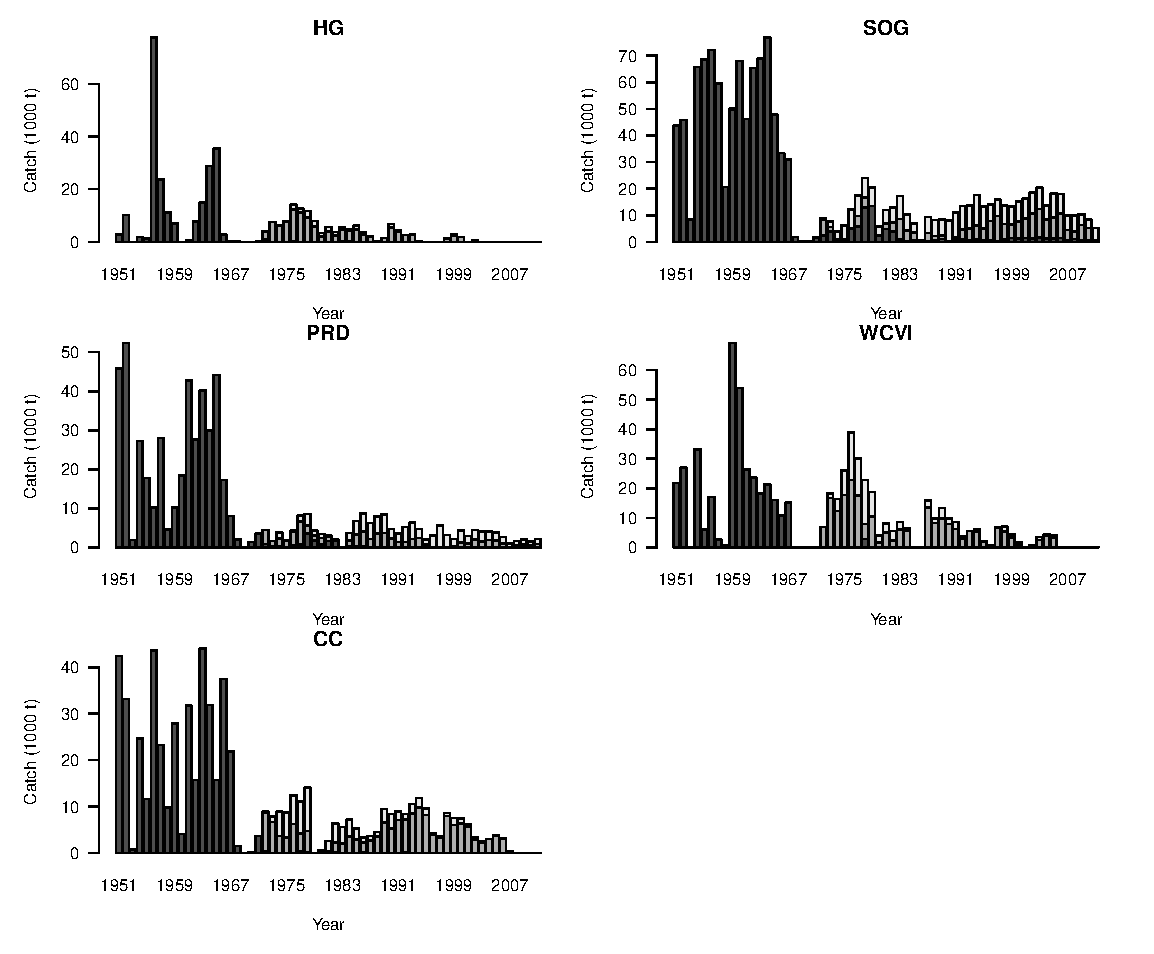
\includegraphics[clip,trim=0 304 300 0 ]
		{../FIGS/iscam_fig_CatchMajorAreas}
		\caption{Catch by gear for Haida Gwaii.}
	\end{figure}
	}
	\only<2>{
	\begin{figure}[htbp]
		\centering
		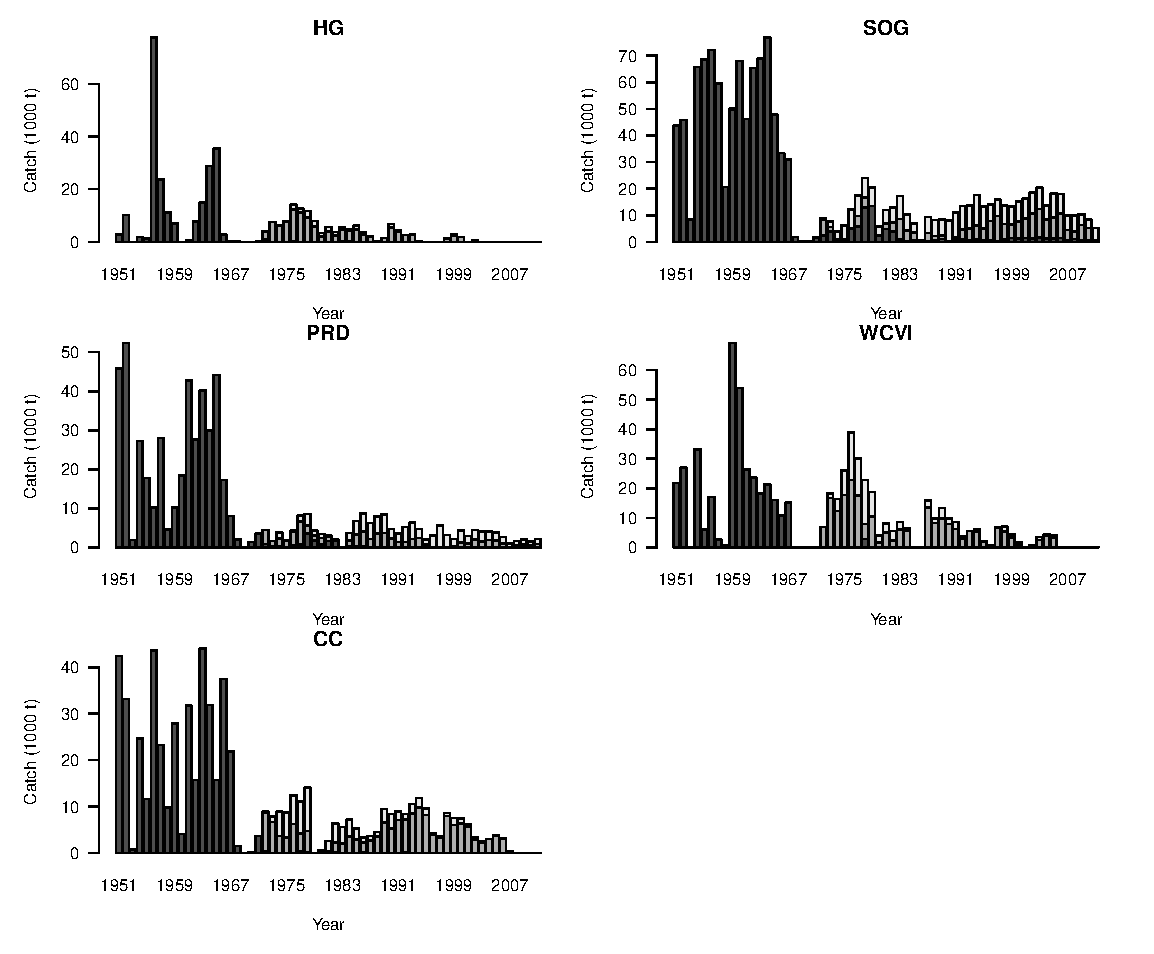
\includegraphics[clip,trim=0 156 300 155 ]
		{../FIGS/iscam_fig_CatchMajorAreas}
		\caption{Catch by gear for Prince Rupert District.}
	\end{figure}
	}
	\only<3>{
	\begin{figure}[htbp]
		\centering
		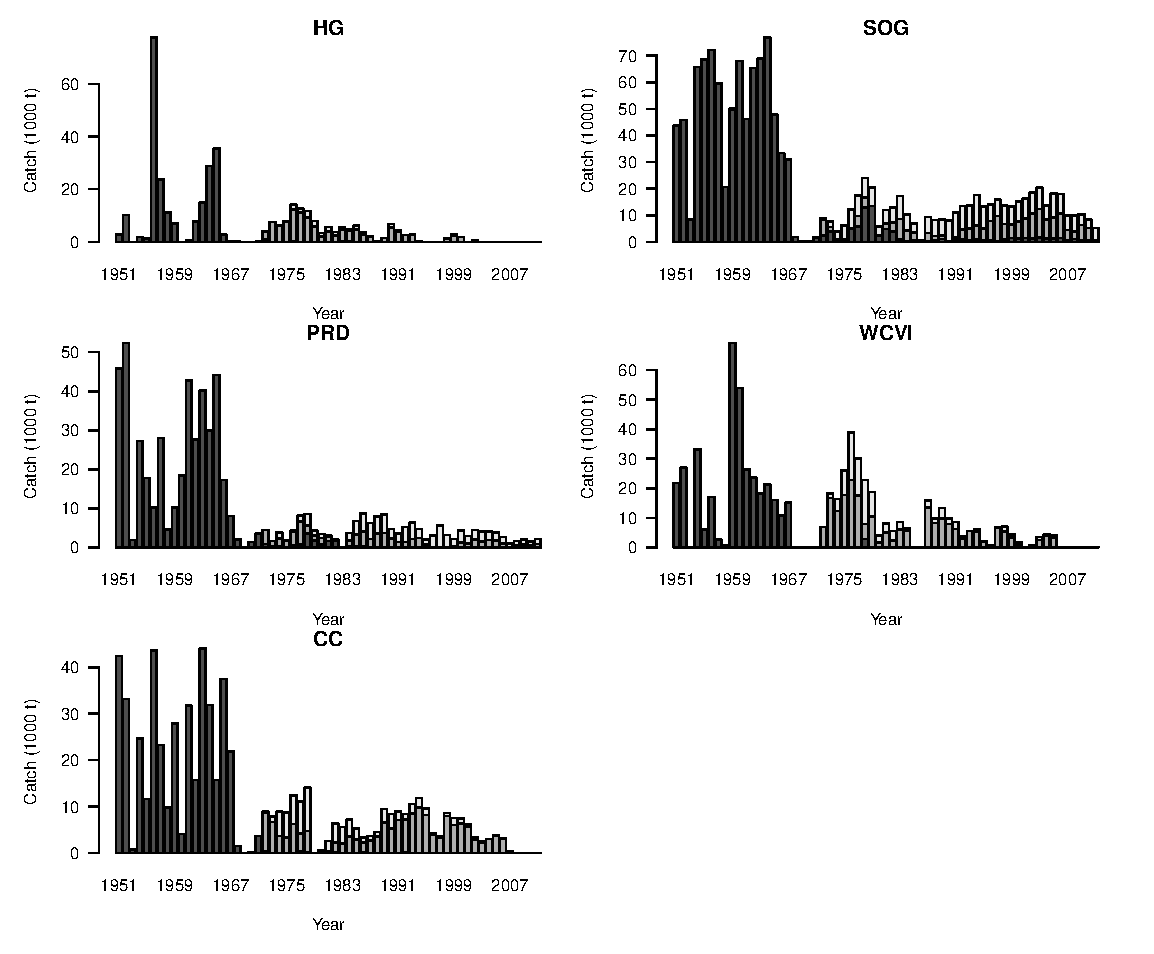
\includegraphics[clip,trim=0 0 300 301 ]
		{../FIGS/iscam_fig_CatchMajorAreas}
		\caption{Catch by gear for Central Coast.}
	\end{figure}
	}
	\only<4>{
	\begin{figure}[htbp]
		\centering
		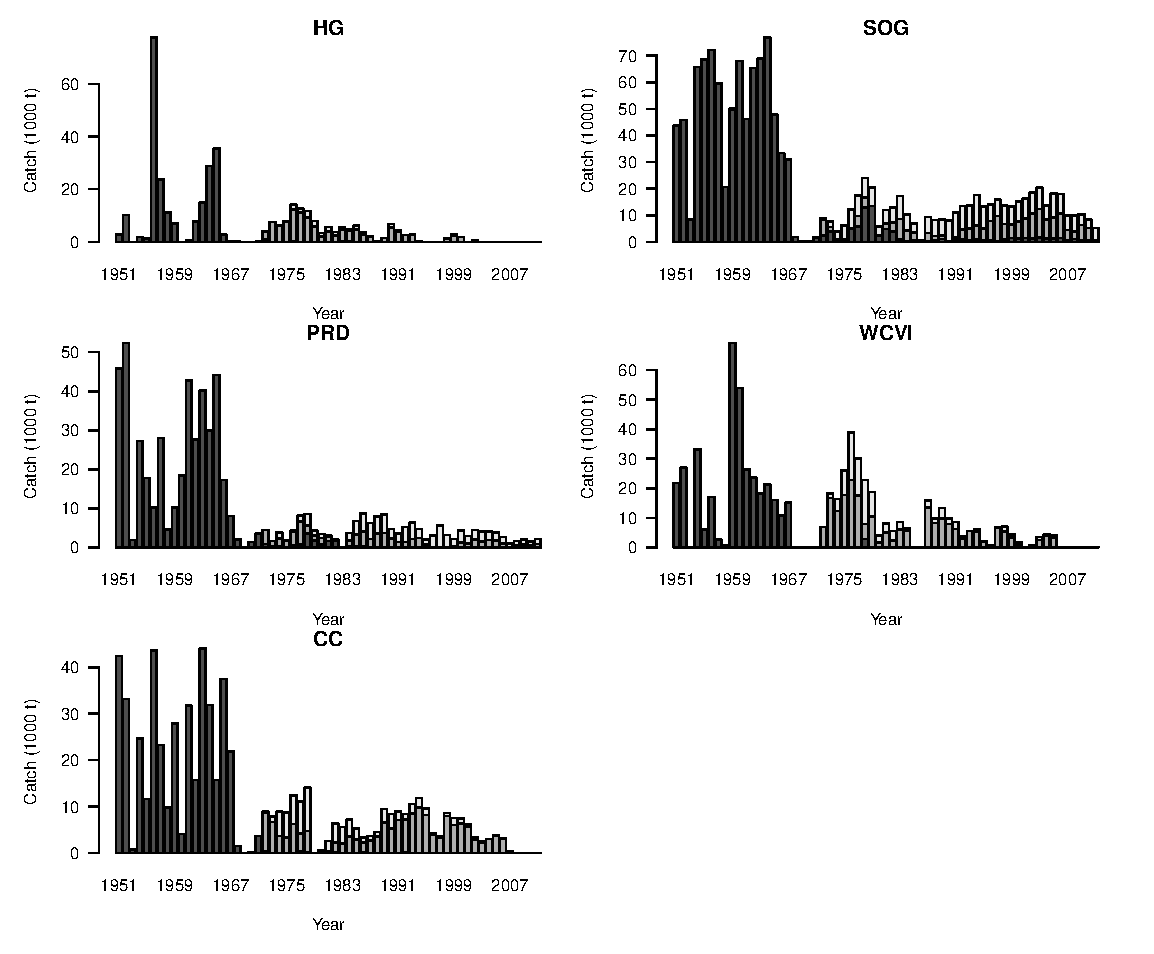
\includegraphics[clip,trim=300 304 0 0 ]
		{../FIGS/iscam_fig_CatchMajorAreas}
		\caption{Catch by gear for Strait of Georgia.}
	\end{figure}
	}
	\only<5>{
	\begin{figure}[htbp]
		\centering
		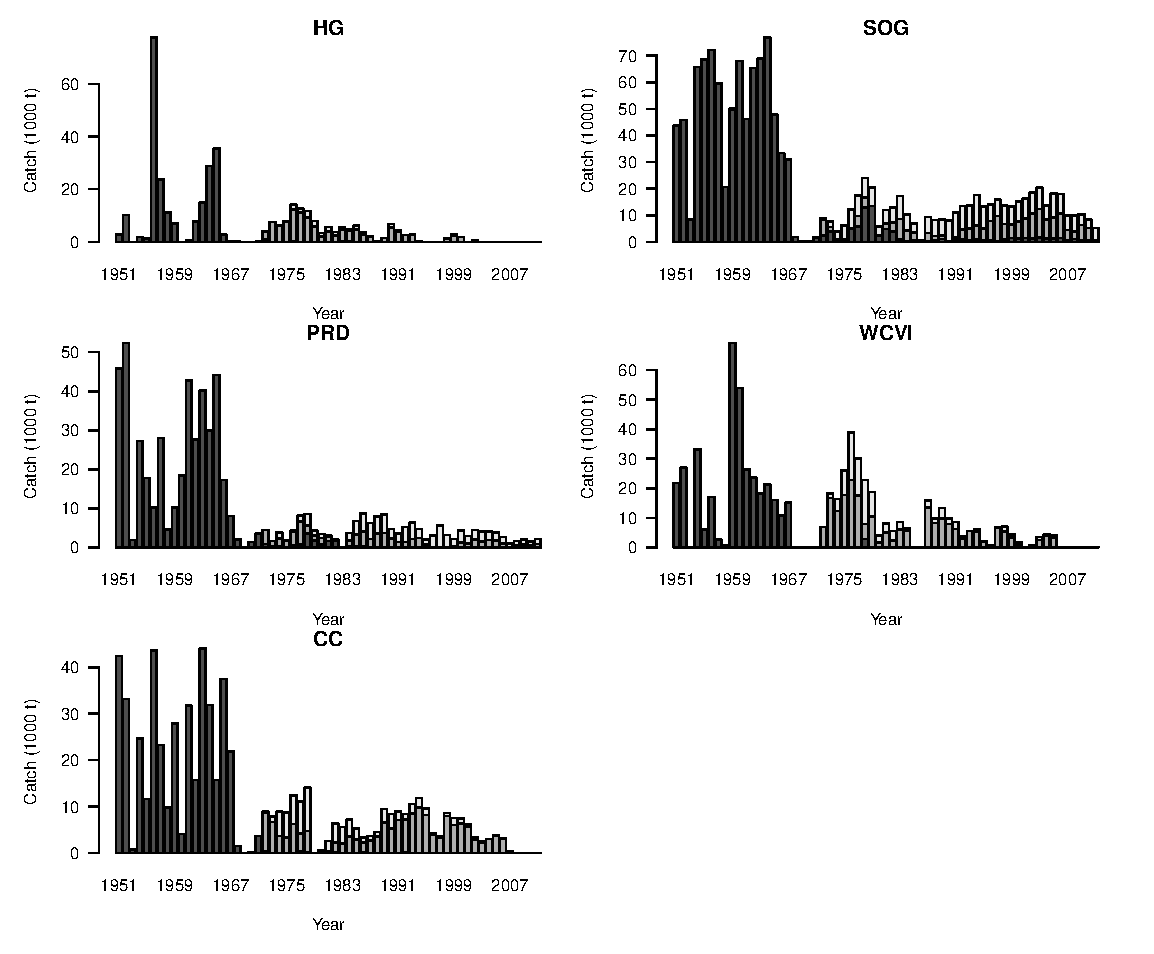
\includegraphics[clip,trim=300 156 0 155 ]
		{../FIGS/iscam_fig_CatchMajorAreas}
		\caption{Catch by gear for West Coast of Vancouver Island.}
	\end{figure}
	}
\end{frame}
%
\begin{frame}[t]\frametitle{Spawning activity in 2010}
	\only<1>{
	\begin{figure}[htbp]
		\centering
		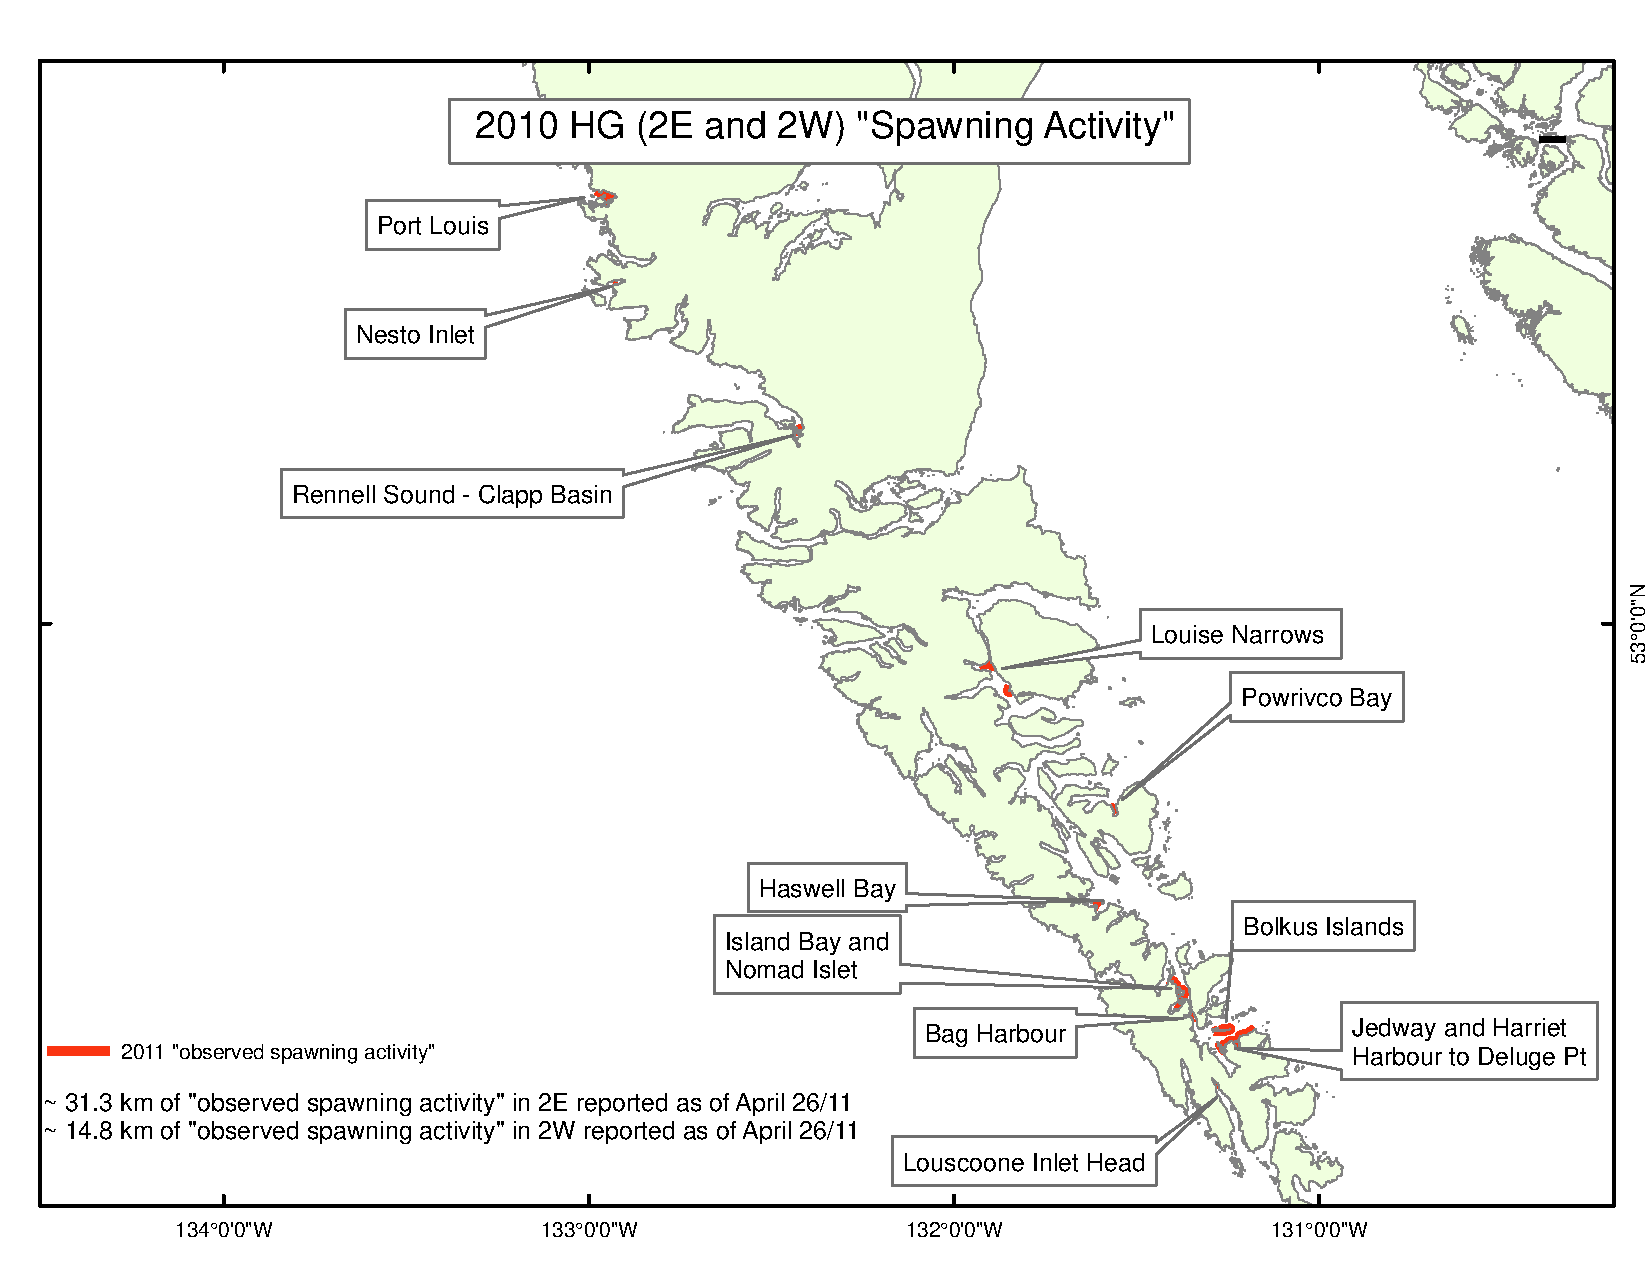
\includegraphics[scale=0.3]
		{../FIGS/PBSfigs/2011-HG-Prelim-WG}
		\caption{2010 Spawning activity in Haida Gwaii.}
	\end{figure}
	}
	\only<2>{
	\begin{figure}[htbp]
		\centering
		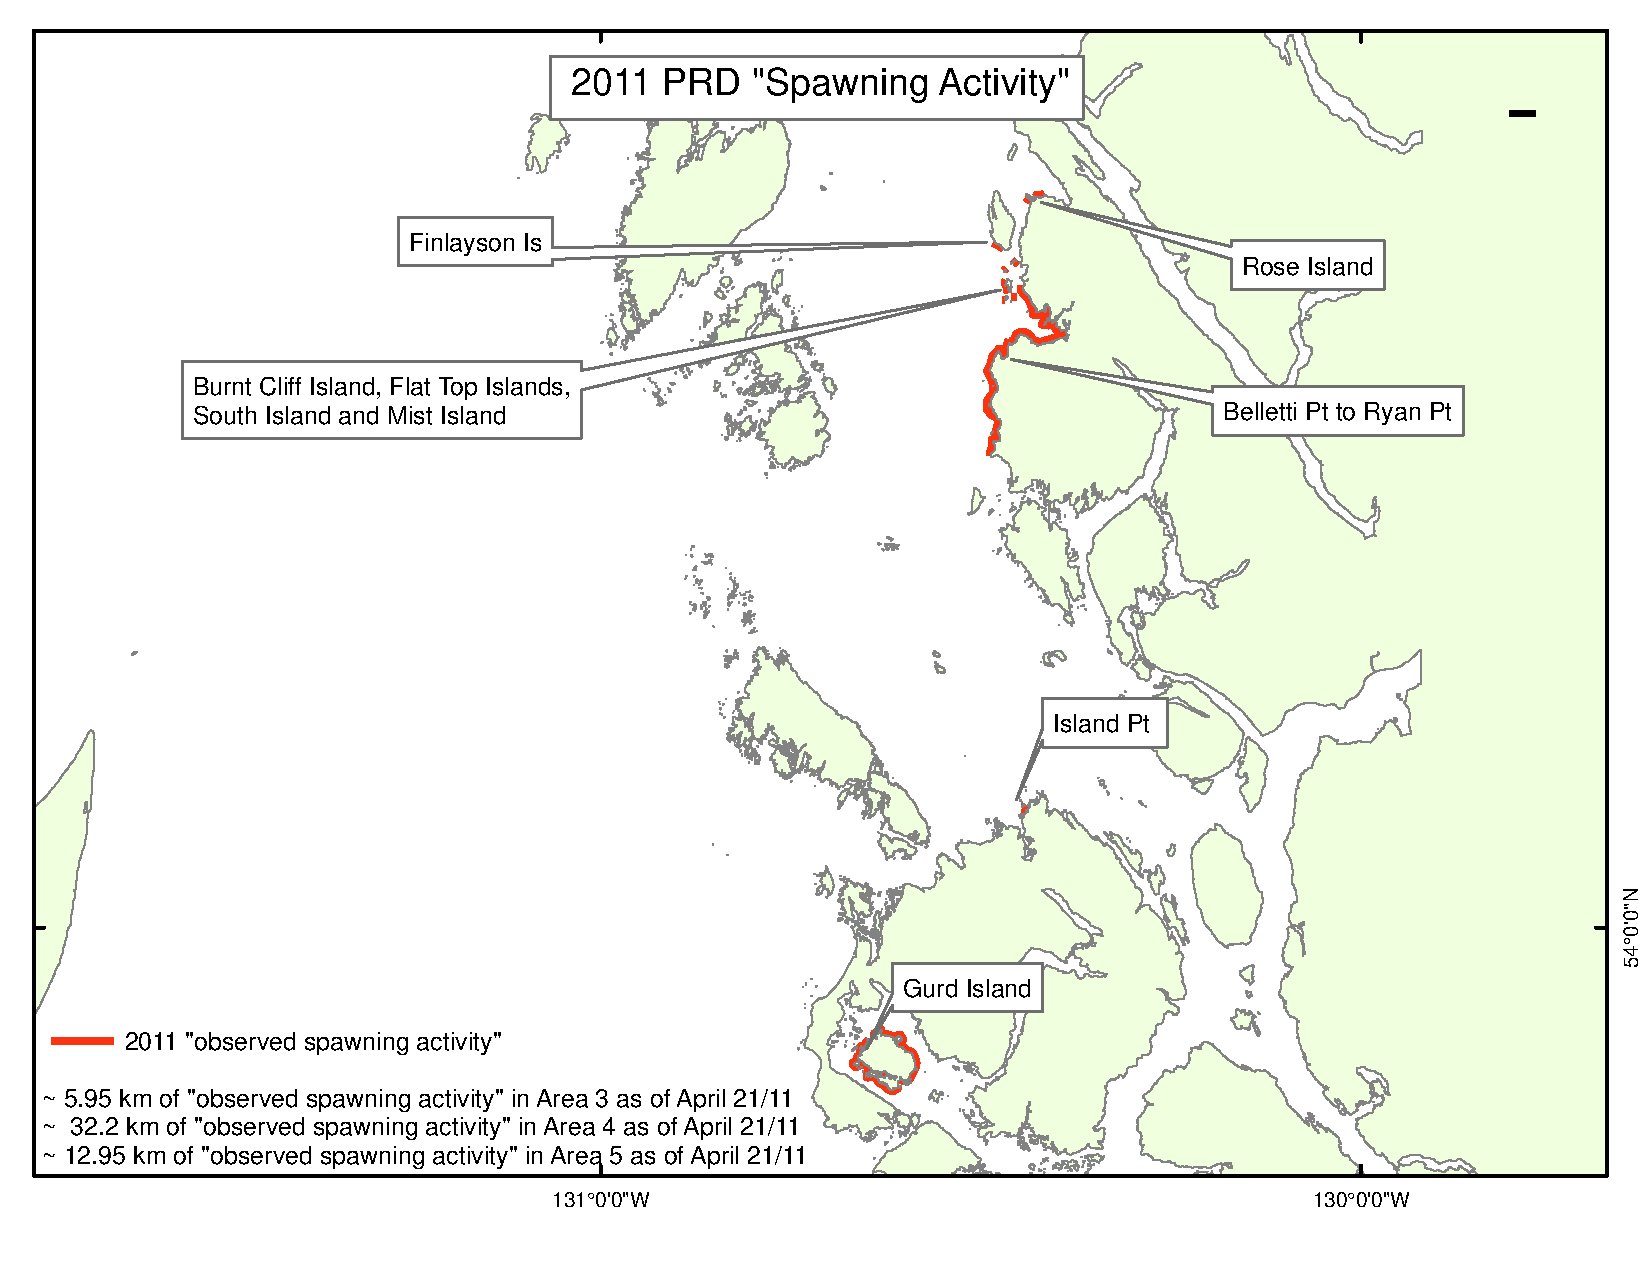
\includegraphics[scale=0.3]
		{../FIGS/PBSfigs/2011-PRD-Prelim-WG}
		\caption{2010 Spawning activity in Prince Rupert District.}
	\end{figure}
	}
	\only<3>{
	\begin{figure}[htbp]
		\centering
		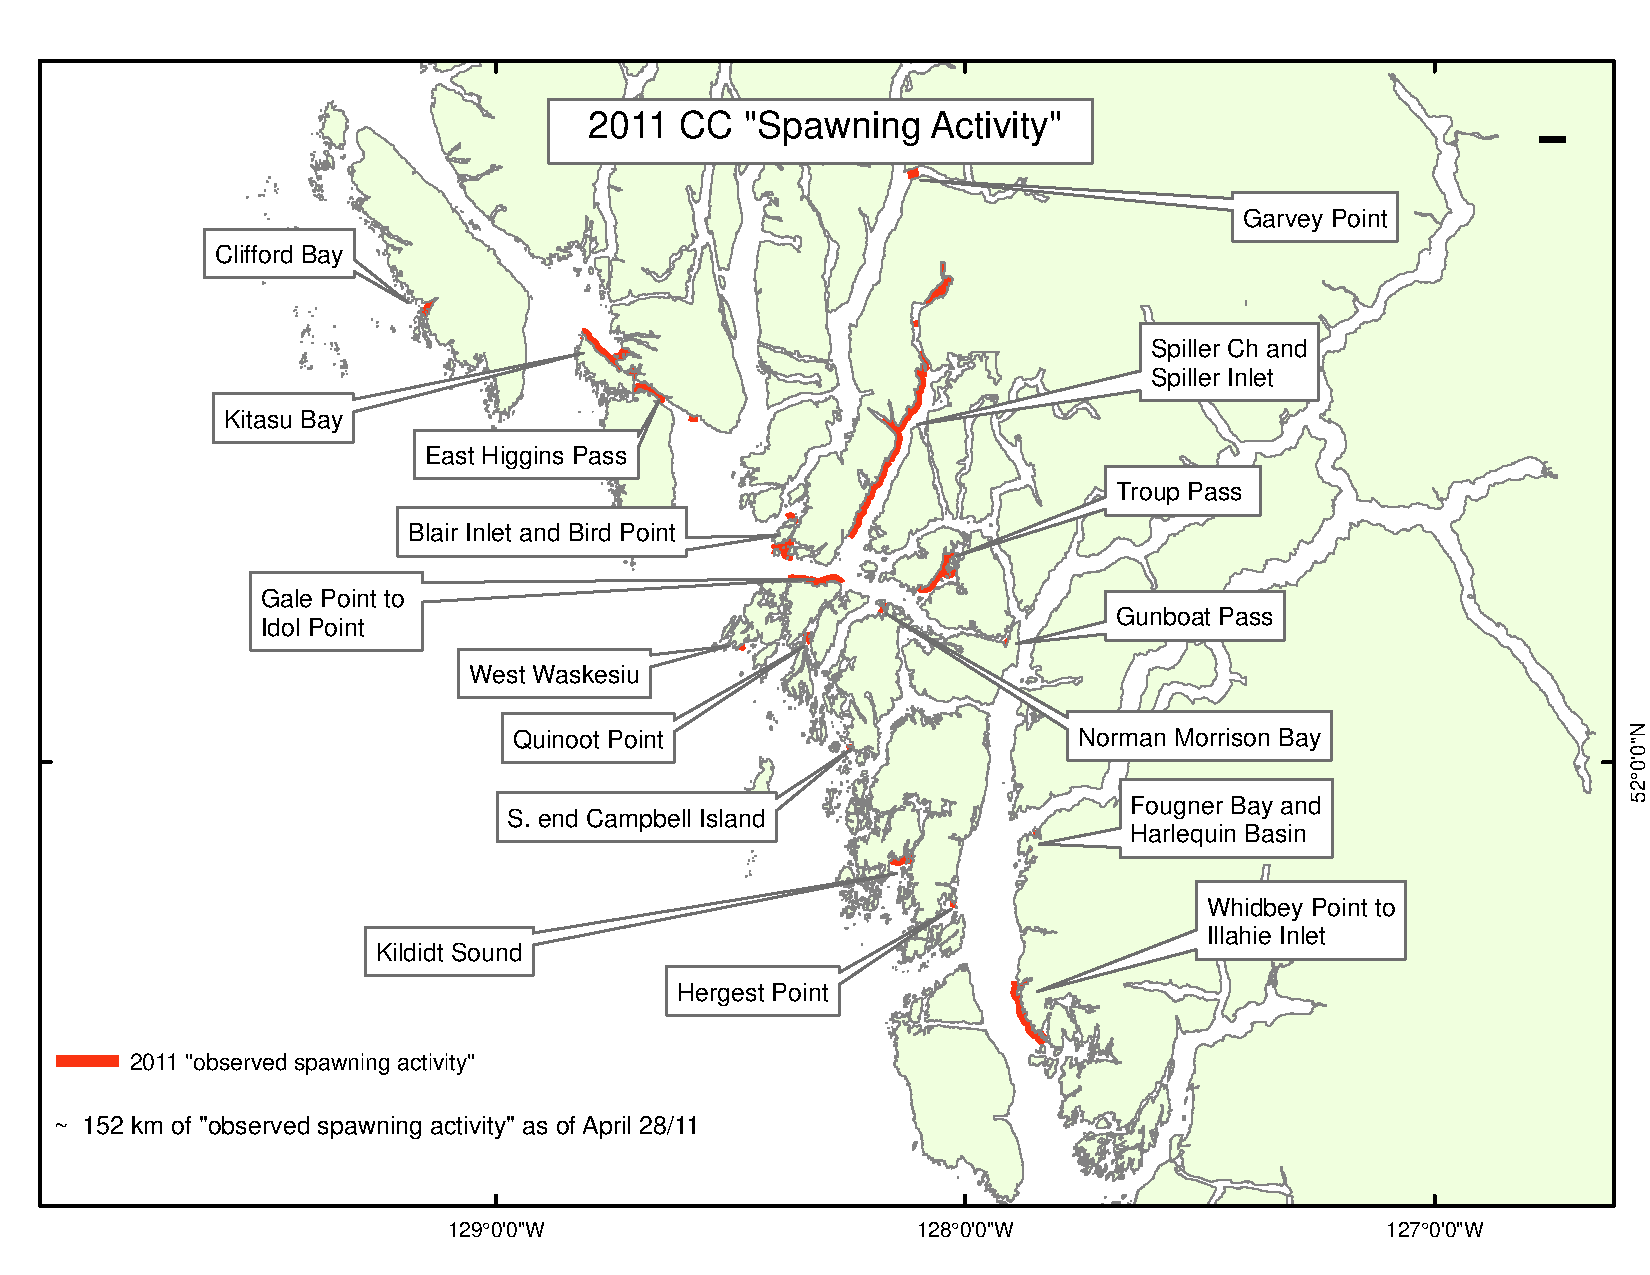
\includegraphics[scale=0.3]
		{../FIGS/PBSfigs/2011-CC-Prelim-WG}
		\caption{2010 Spawning activity in Central Coast.}
	\end{figure}
	}
	\only<4>{
	\begin{figure}[htbp]
		\centering
		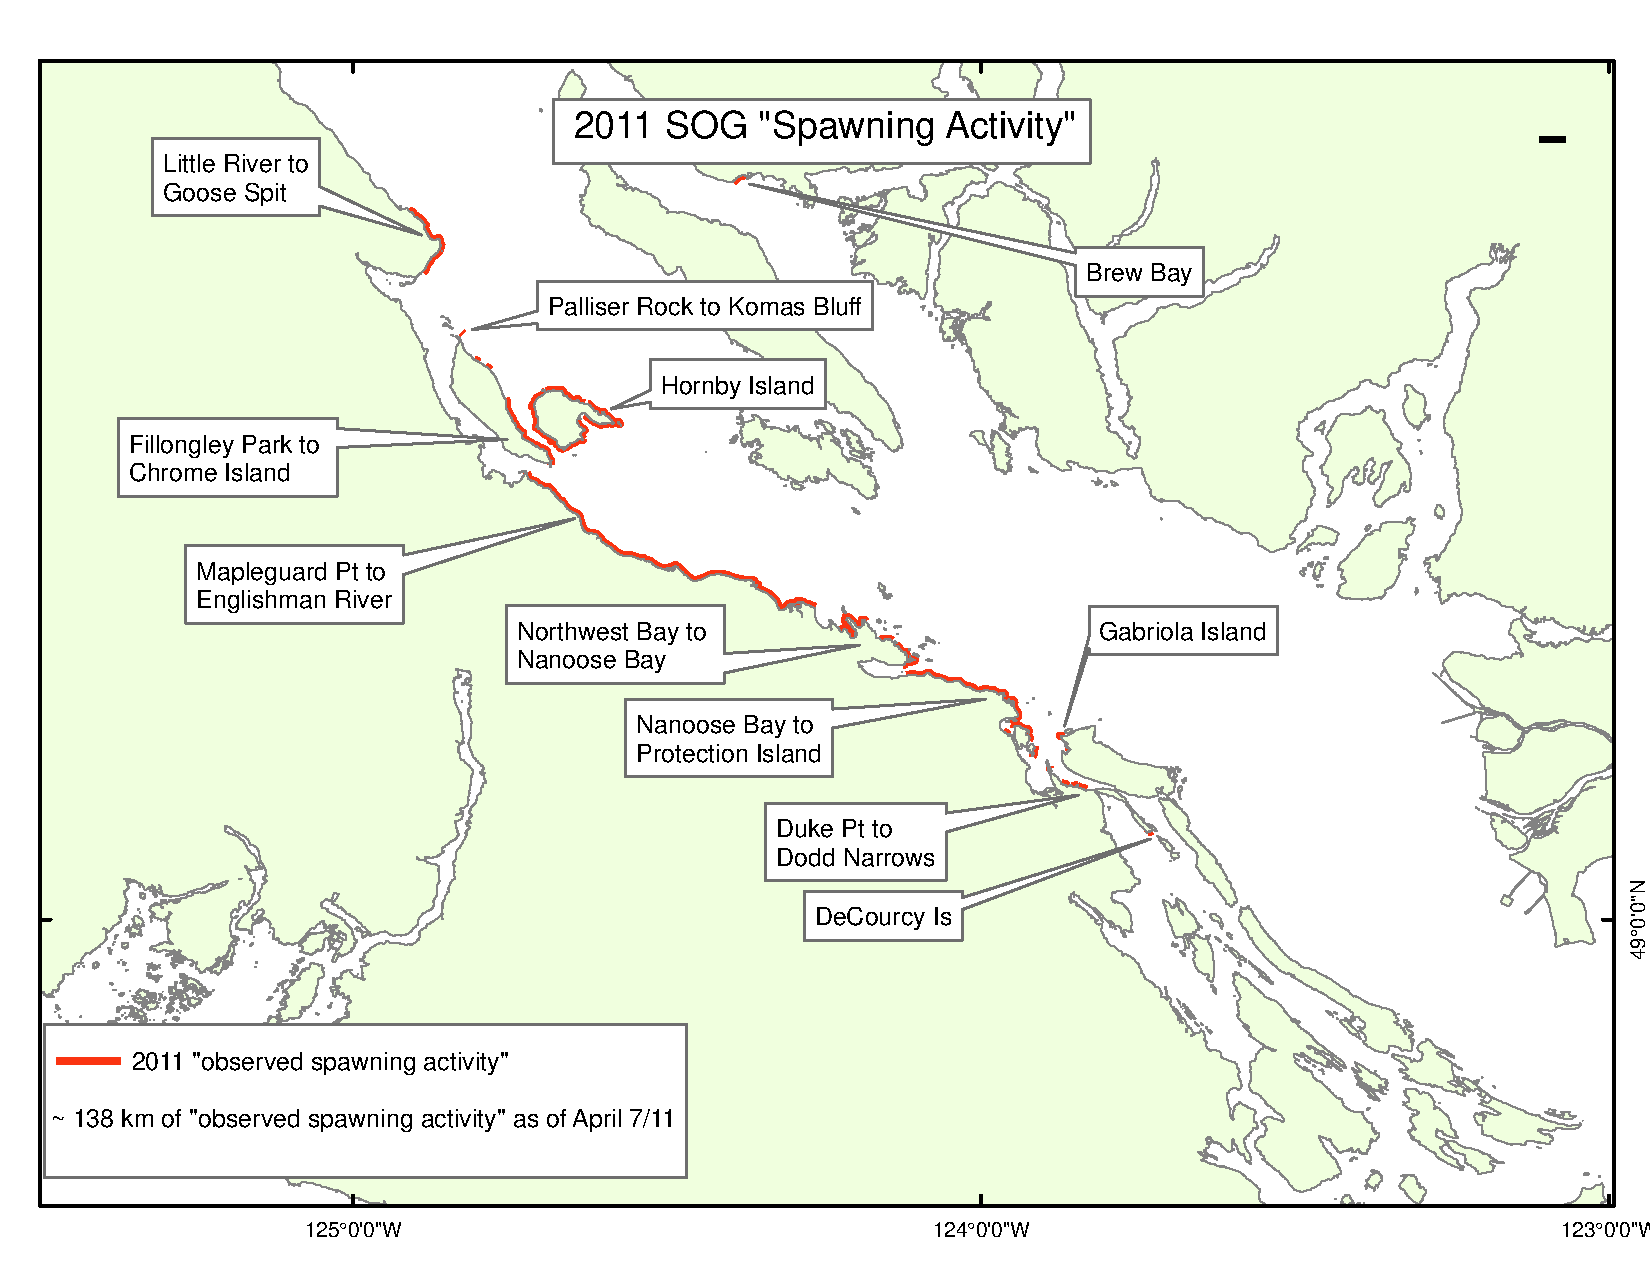
\includegraphics[scale=0.3]
		{../FIGS/PBSfigs/2011-SOG-Prelim-WG}
		\caption{2010 Spawning activity in Strait of Georgia.}
	\end{figure}
	}
	\only<5>{
	\begin{figure}[htbp]
		\centering
		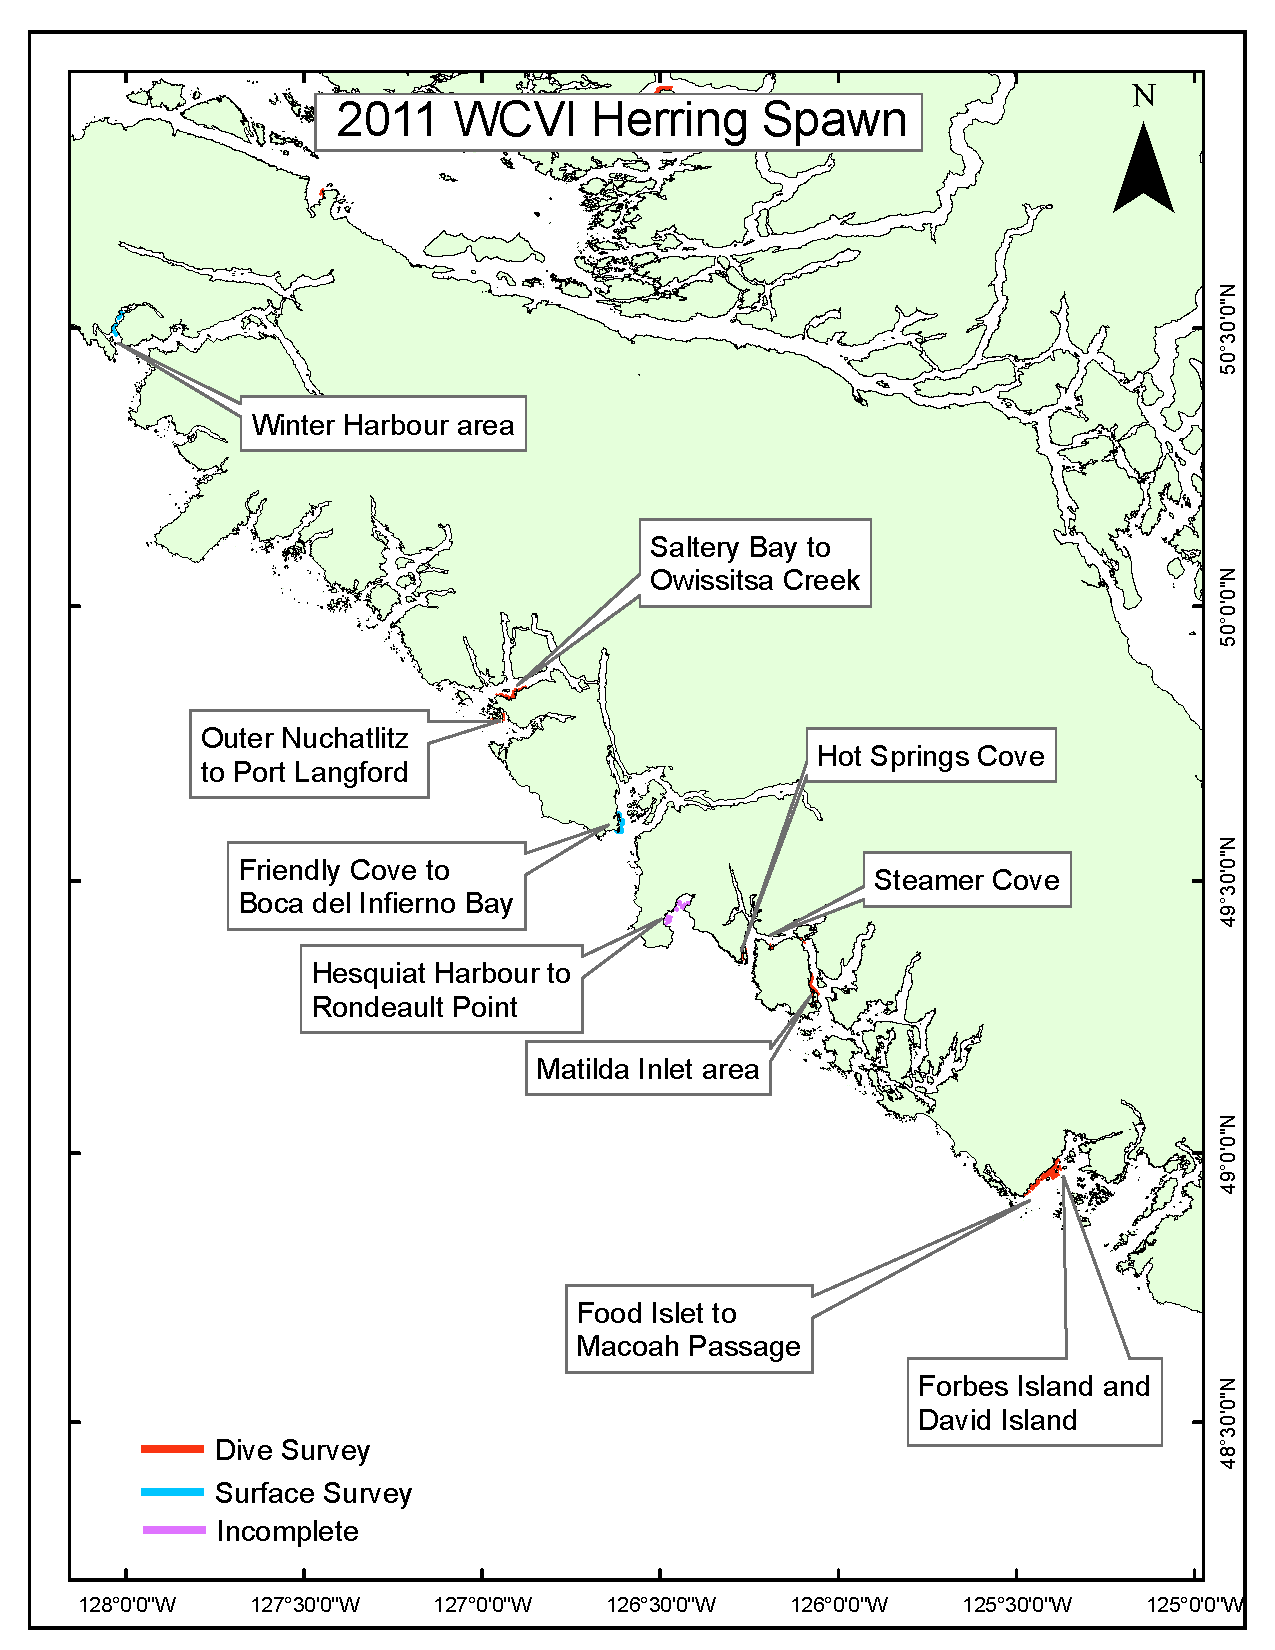
\includegraphics[scale=0.23]
		{../FIGS/PBSfigs/2011_spawn_WCVI_August16}
		\caption{2010 Spawning activity in West Coast Vancouver Island.}
	\end{figure}
	}
\end{frame}
%
\begin{frame}[t]\frametitle{Spawn survey time series}
	\only<1>{
	\begin{figure}[htbp]
		\centering
		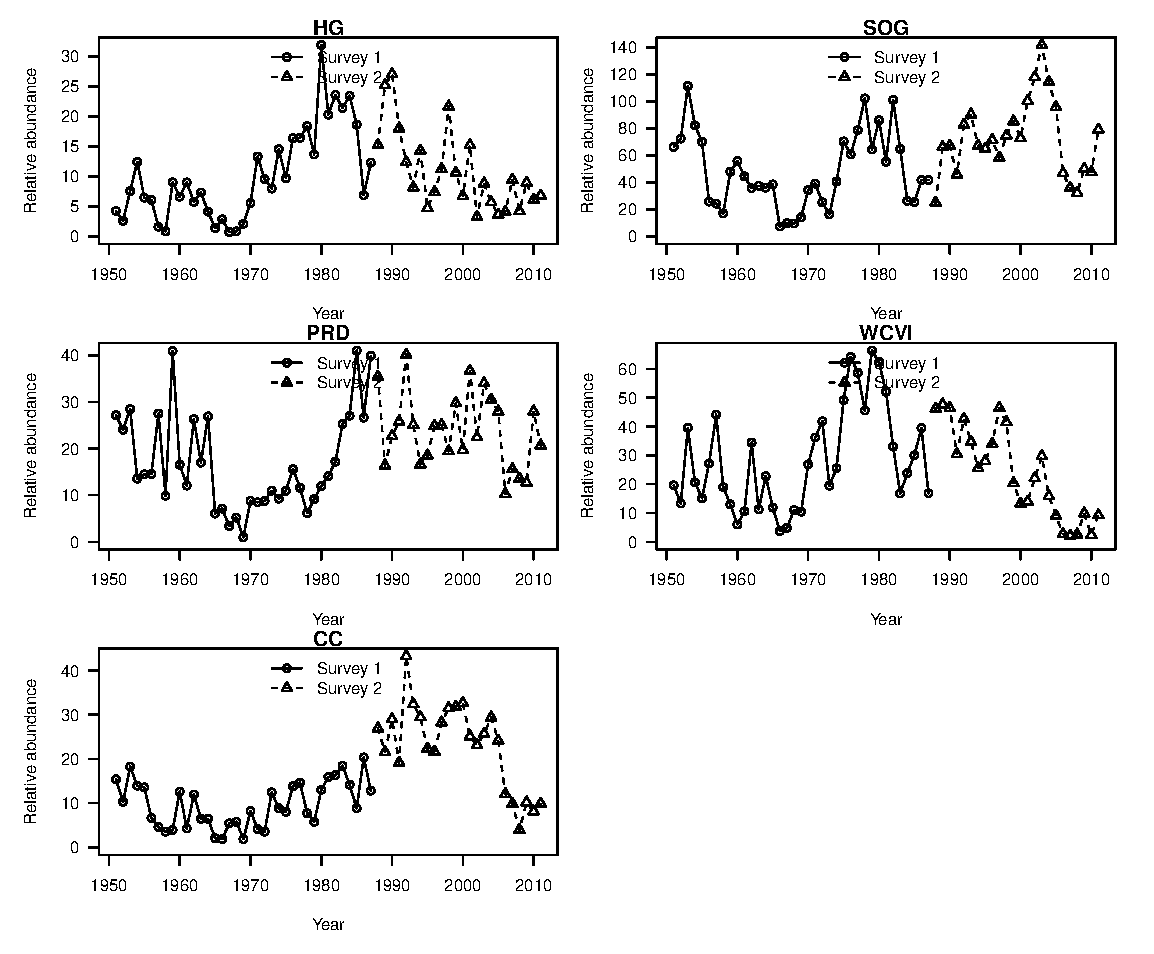
\includegraphics[clip,trim=0 304 275 0]
		{../FIGS/iscam_fig_SurveyMajorAreas}
		\caption{Spawn survey series in Haida Gwaii.}
	\end{figure}
	}
	%
	\only<2>{
	\begin{figure}[htbp]
		\centering
		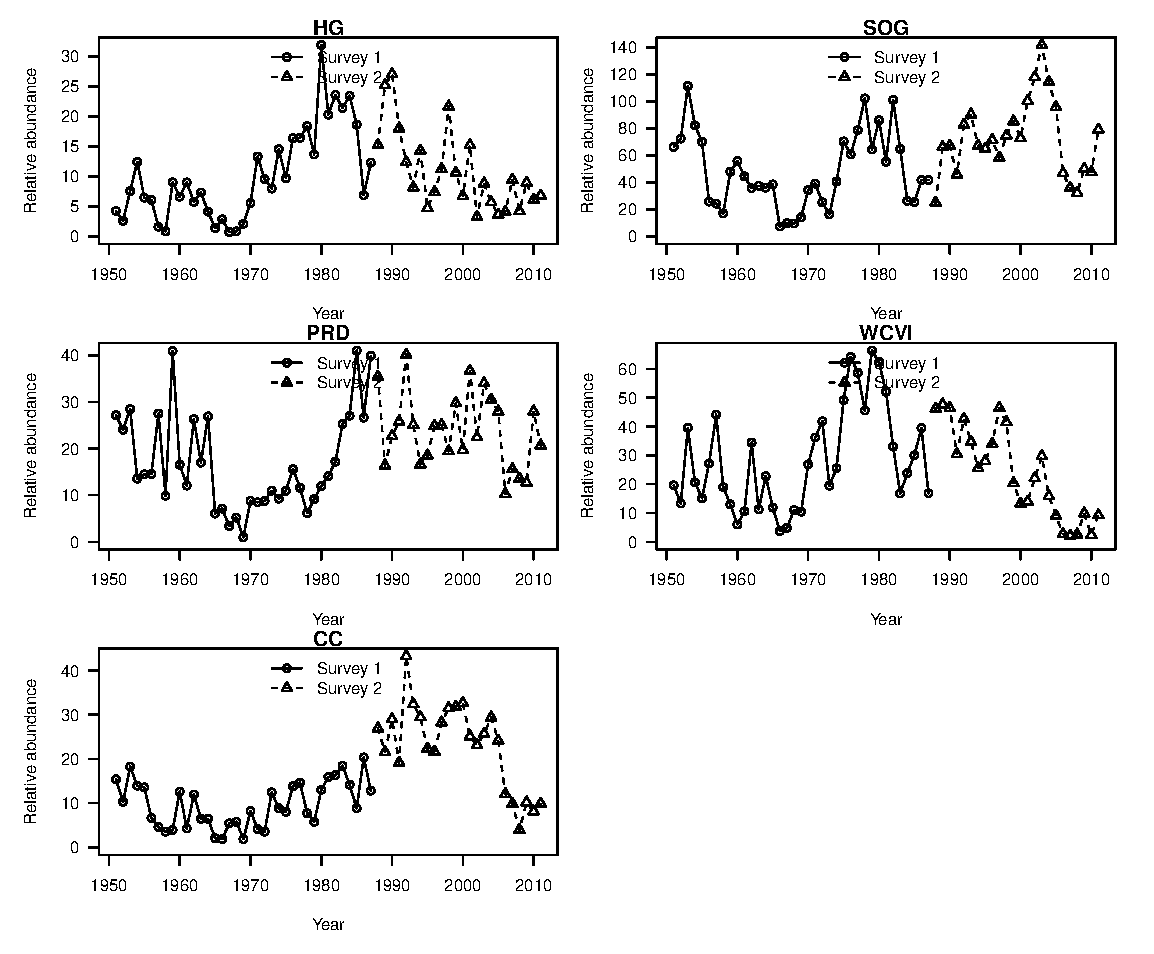
\includegraphics[clip,trim=0 156 275 155]
		{../FIGS/iscam_fig_SurveyMajorAreas}
		\caption{Spawn survey series in Prince Rupert District.}
	\end{figure}
	}
	%
	\only<3>{
	\begin{figure}[htbp]
		\centering
		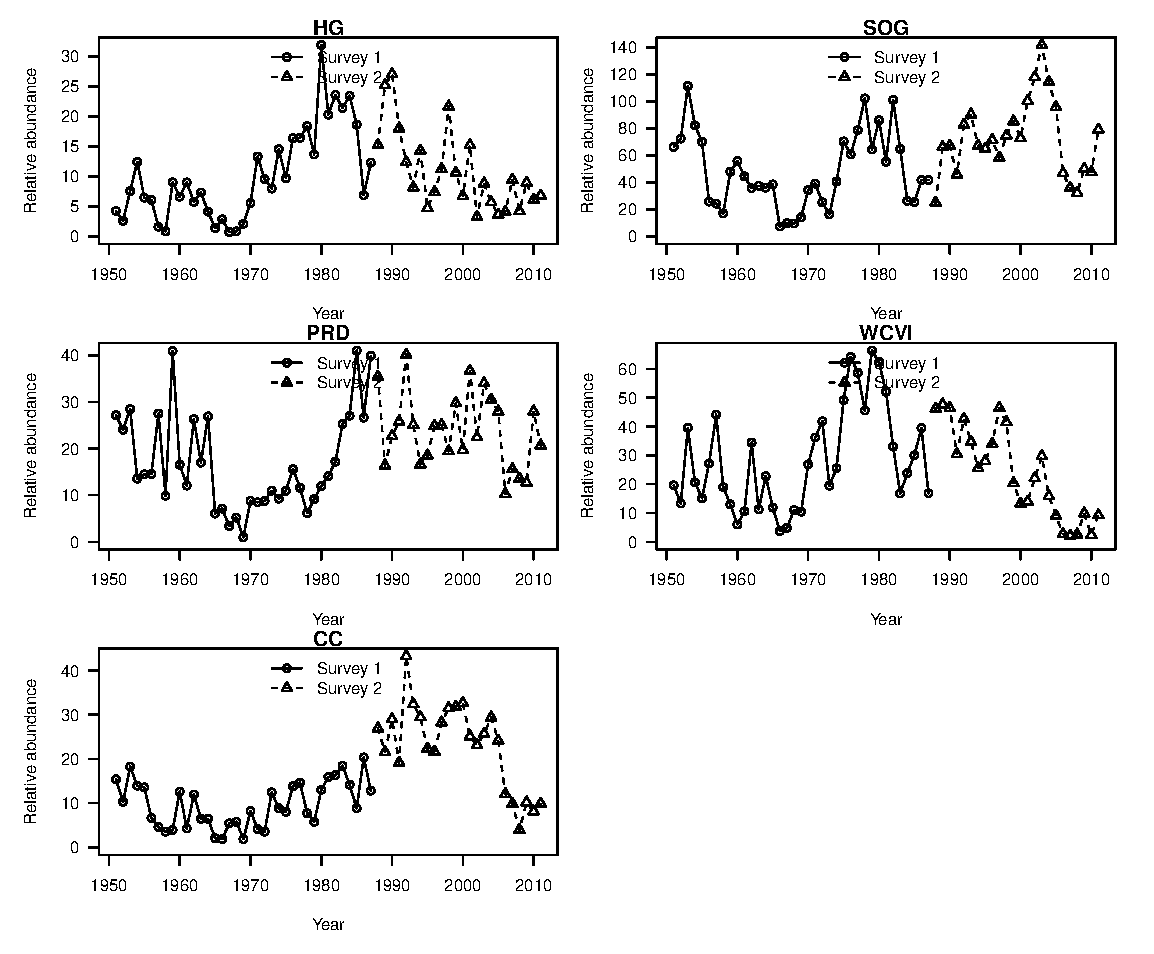
\includegraphics[clip,trim=0 0 275 301]
		{../FIGS/iscam_fig_SurveyMajorAreas}
		\caption{Spawn survey series in Central Coast.}
	\end{figure}
	}
	%
	\only<4>{
	\begin{figure}[htbp]
		\centering
		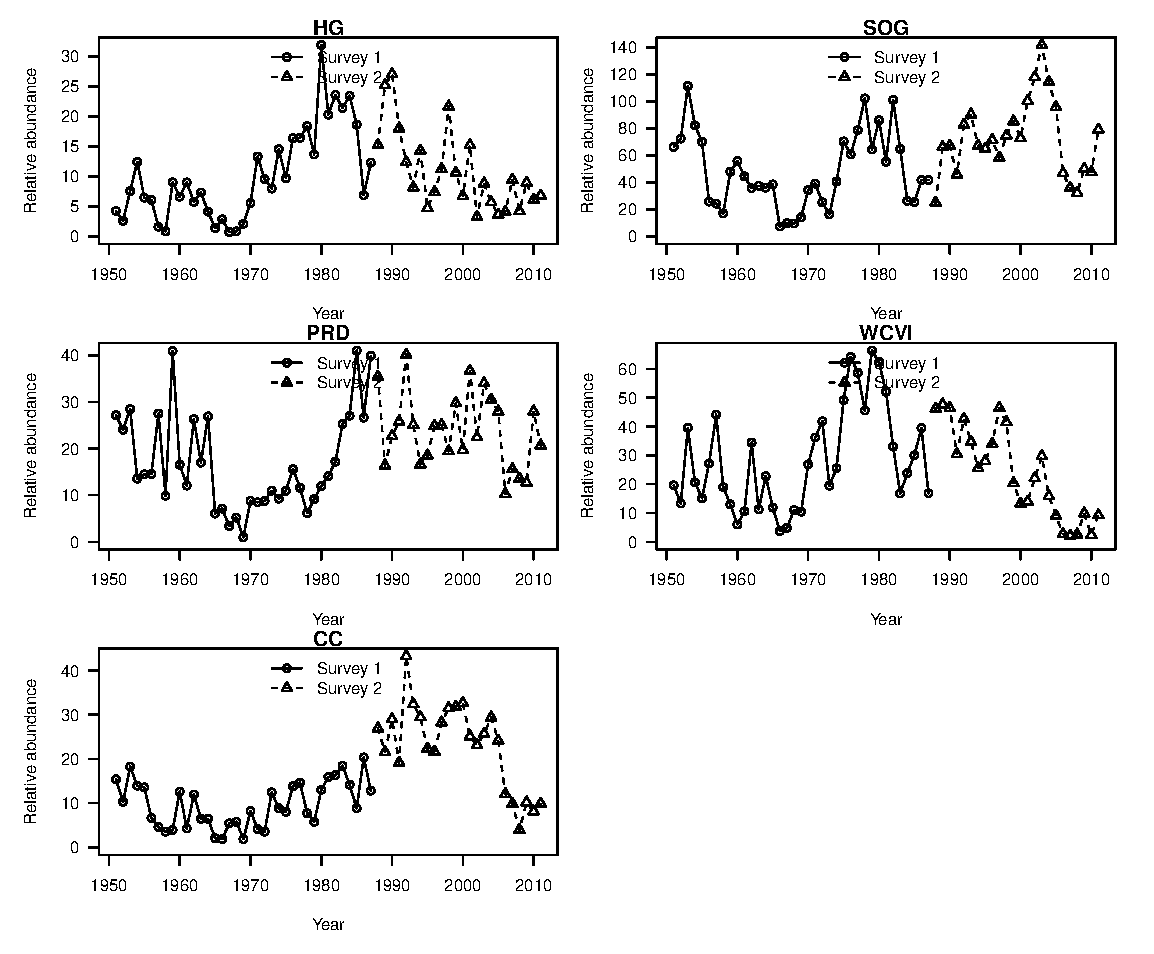
\includegraphics[clip,trim=275 304 0 0]
		{../FIGS/iscam_fig_SurveyMajorAreas}
		\caption{Spawn survey series in Strait of Georgia.}
	\end{figure}
	}
	%
	\only<5>{
	\begin{figure}[htbp]
		\centering
		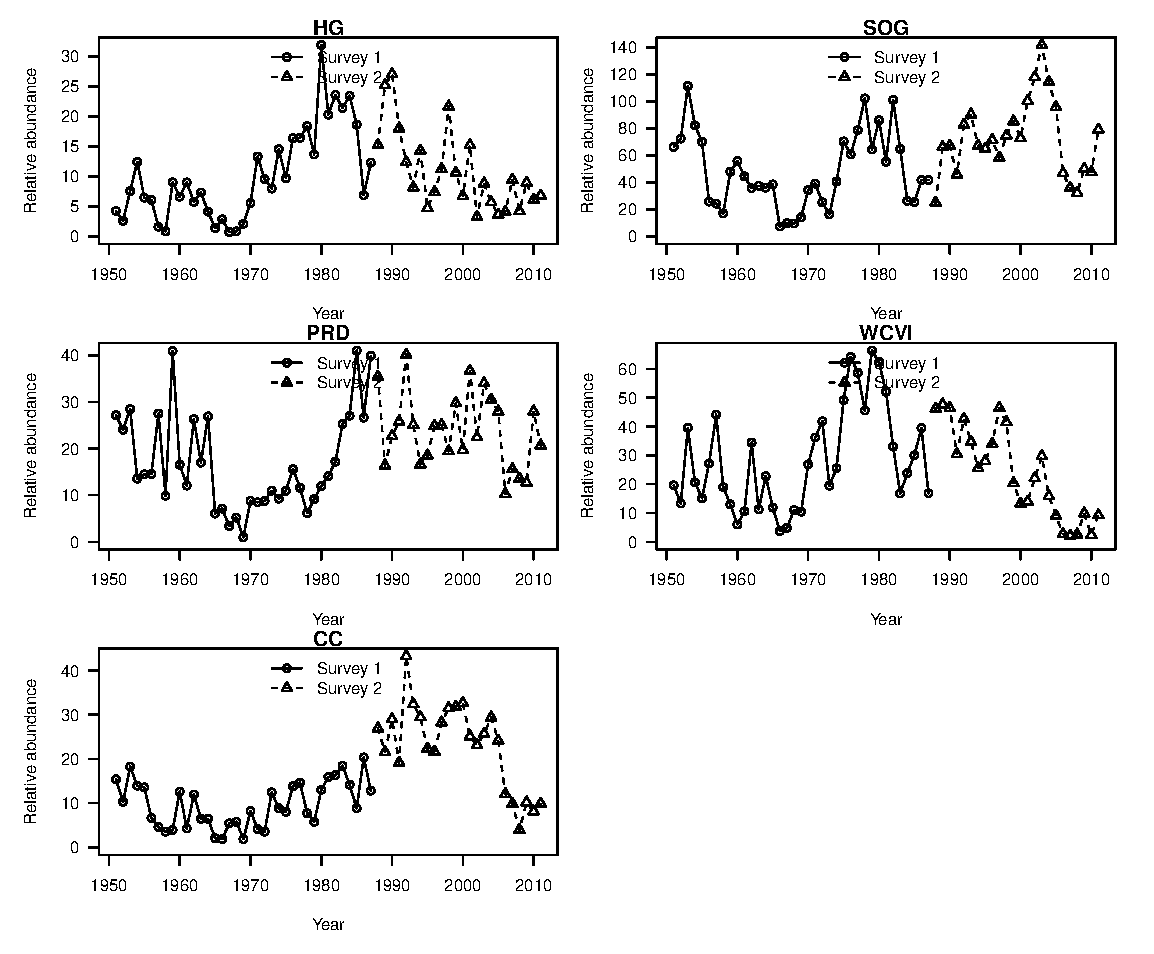
\includegraphics[clip,trim=275 156 0 155]
		{../FIGS/iscam_fig_SurveyMajorAreas}
		\caption{Spawn survey series in West Coast of Vancouver Island.}
	\end{figure}
	}
\end{frame}
%
\begin{frame}[t]\frametitle{Age-composition data}
	\only<1>{
	\begin{figure}[htbp]
		\centering
		\vspace{-0.5cm}	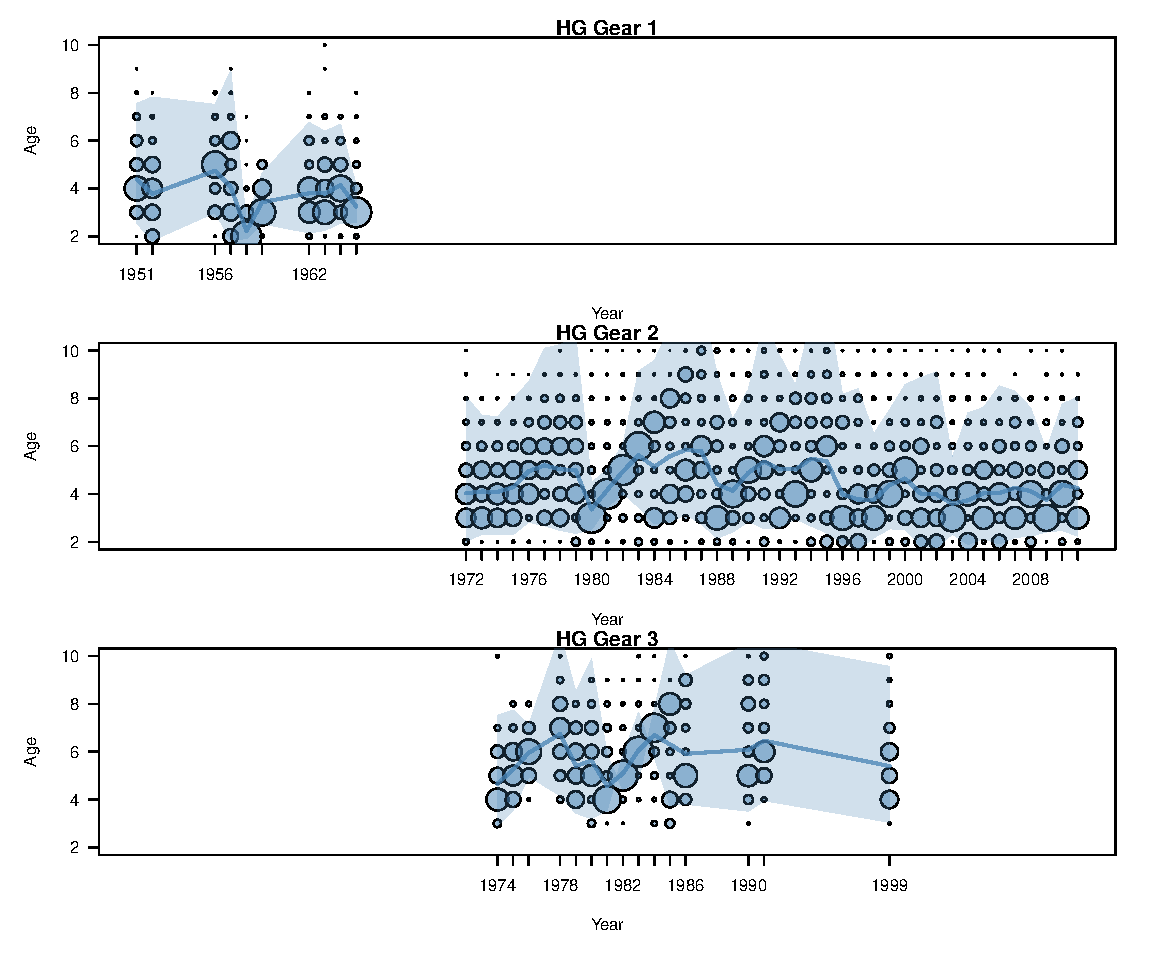
\includegraphics
		[height=0.85\textheight,width=\textwidth]
		{../FIGS/iscam_fig_AgeCompsHG}
		\vspace{-1cm}
		\caption{Haida Gwaii: winter seine, seine-roe, gillnet.}
	\end{figure}
	}
	%
	\only<2>{
	\begin{figure}[htbp]
		\centering
		\vspace{-0.5cm}	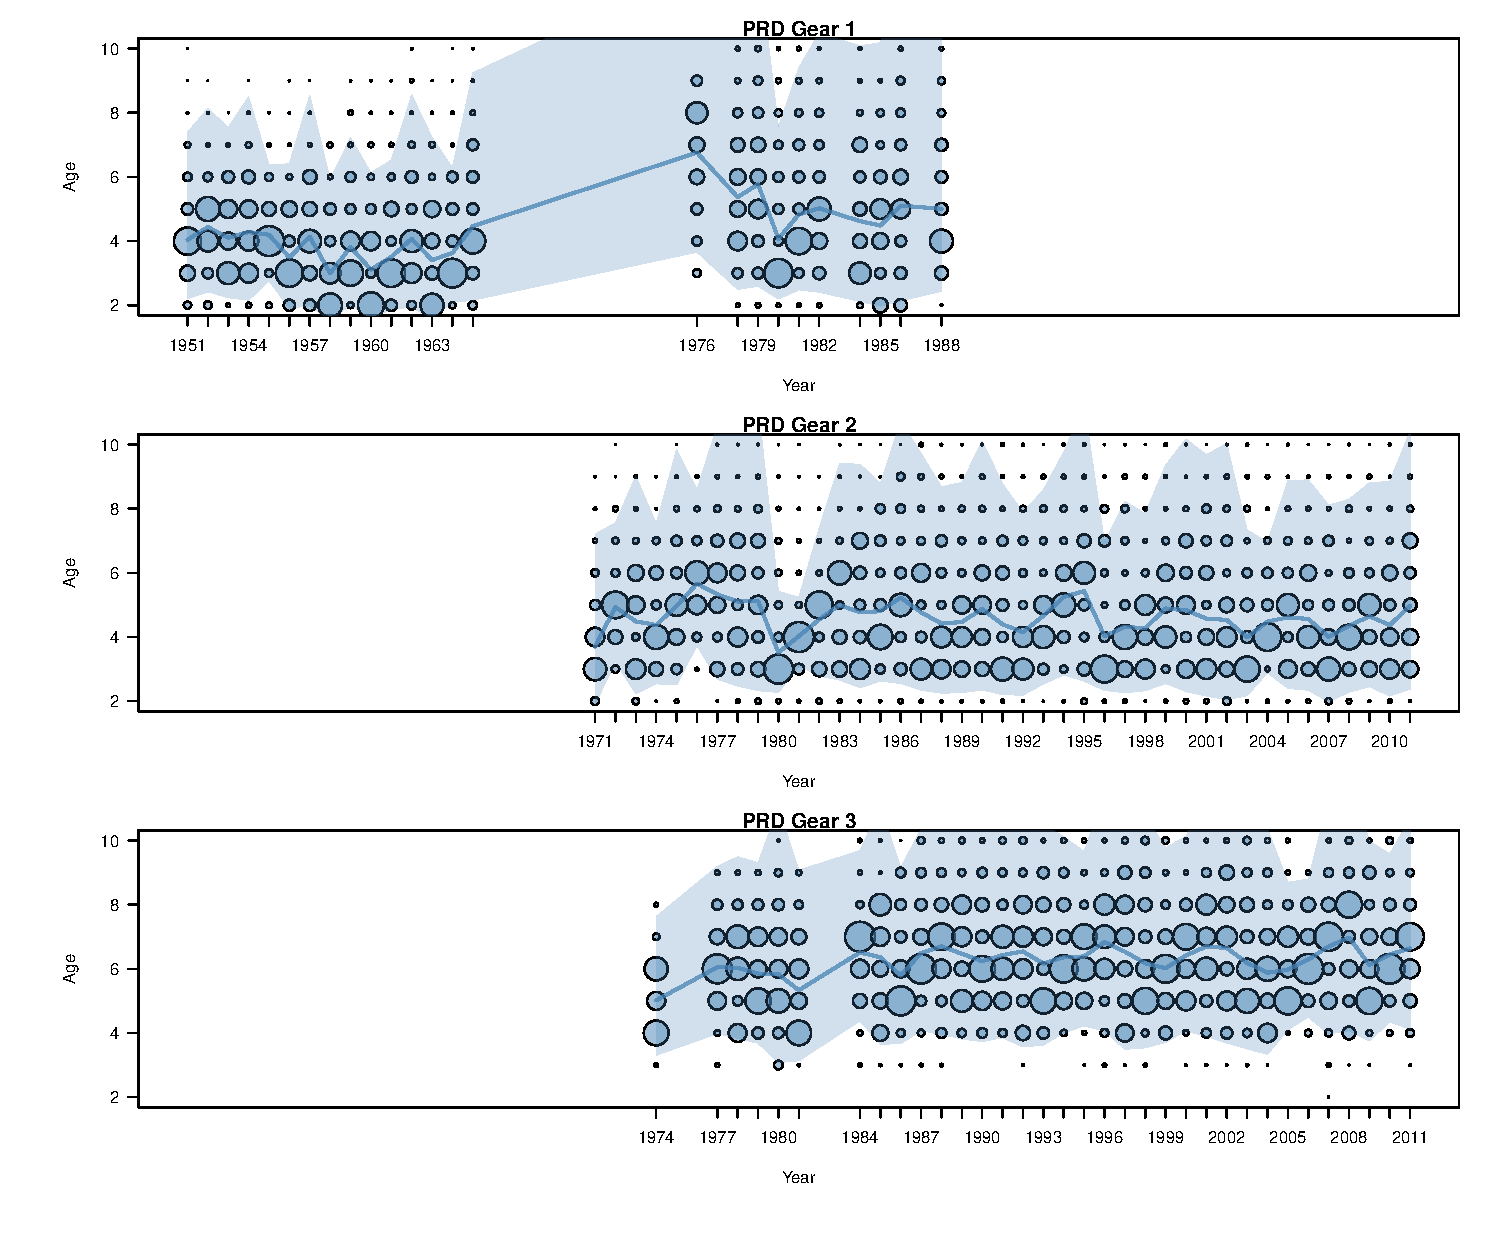
\includegraphics
		[height=0.85\textheight,width=\textwidth]
		{../FIGS/iscam_fig_AgeCompsPRD}
		\vspace{-1cm}
		\caption{Prince Rupert District: winter seine, seine-roe, gillnet.}
	\end{figure}
	}
	%
	\only<3>{
	\begin{figure}[htbp]
		\centering
		\vspace{-0.5cm}	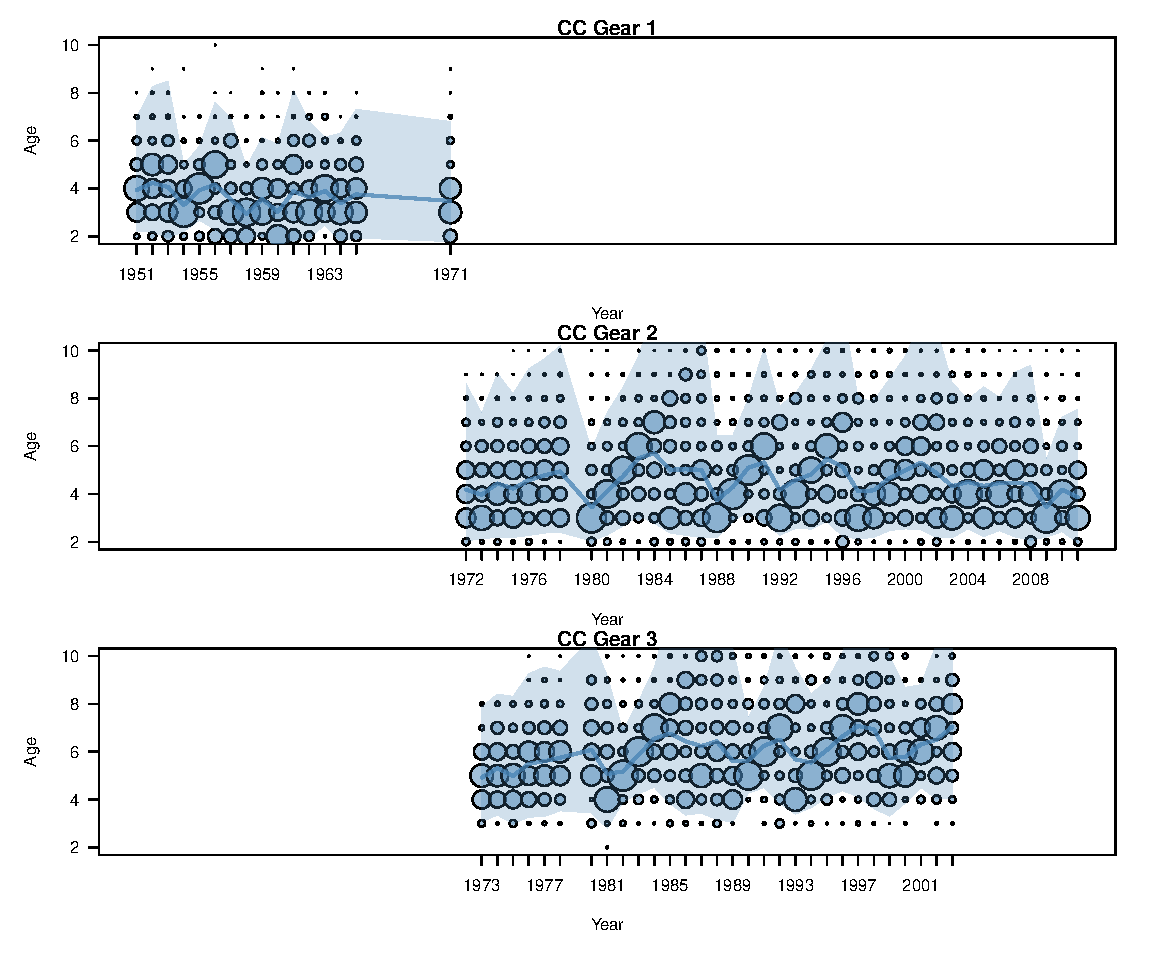
\includegraphics
		[height=0.85\textheight,width=\textwidth]
		{../FIGS/iscam_fig_AgeCompsCC}
		\vspace{-1cm}
		\caption{Central Coast: winter seine, seine-roe, gillnet.}
	\end{figure}
	}
	%
	\only<4>{
	\begin{figure}[htbp]
		\centering
		\vspace{-0.5cm}	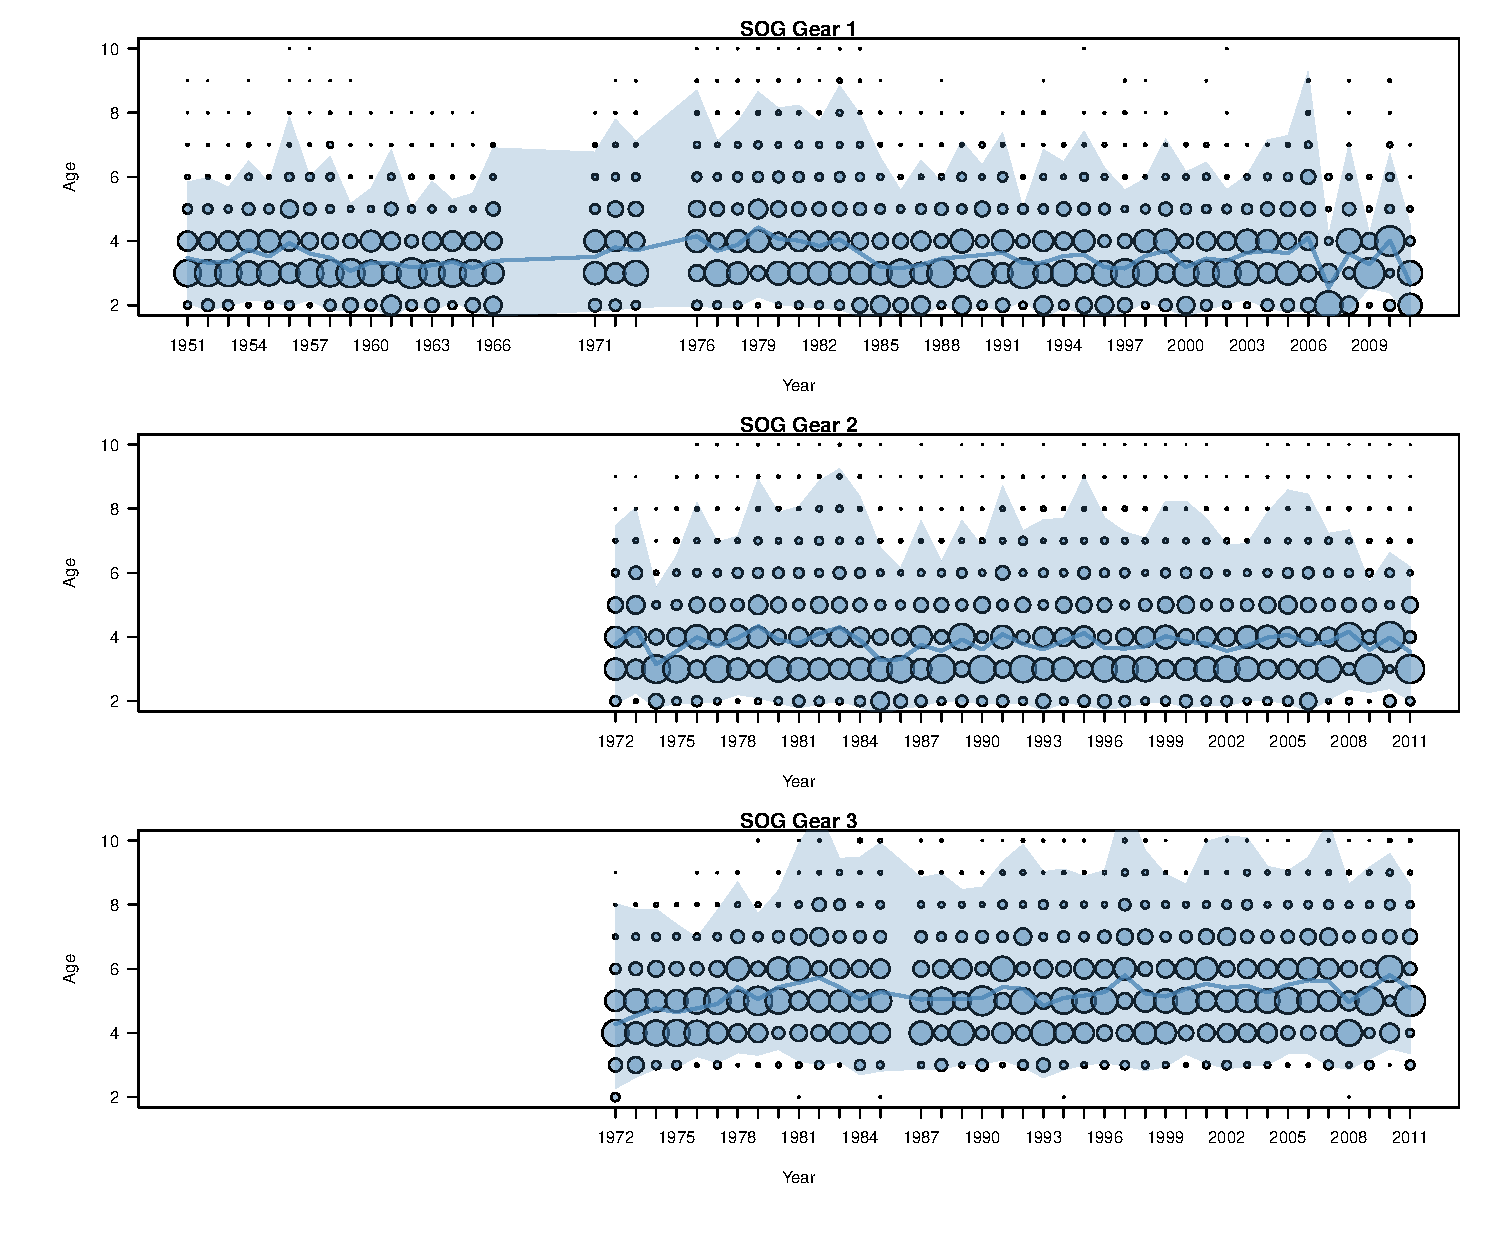
\includegraphics
		[height=0.85\textheight,width=\textwidth]
		{../FIGS/iscam_fig_AgeCompsSOG}
		\vspace{-1cm}
		\caption{Strait of Georgia: winter seine, seine-roe, gillnet.}
	\end{figure}
	}
	%
	\only<5>{
	\begin{figure}[htbp]
		\centering
		\vspace{-0.5cm}	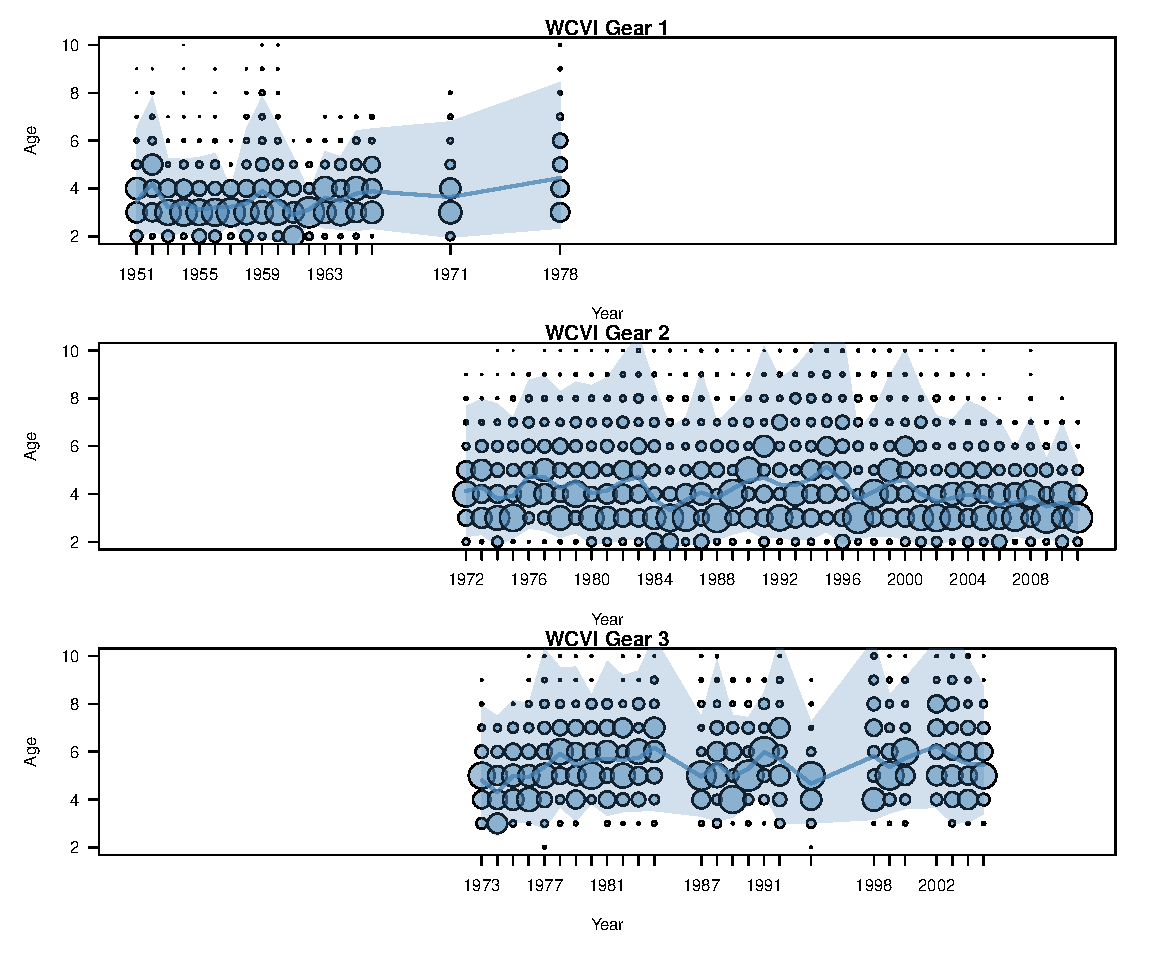
\includegraphics
		[height=0.85\textheight,width=\textwidth]
		{../FIGS/iscam_fig_AgeCompsWCVI}
		\vspace{-1cm}
		\caption{West Coast Vancouver Island: winter seine, seine-roe, gillnet.}
	\end{figure}
	}
	
\end{frame}
%
\begin{frame}[t]\frametitle{Weight-at-age}
	\only<1>{
	\begin{figure}[htbp]
		\centering
		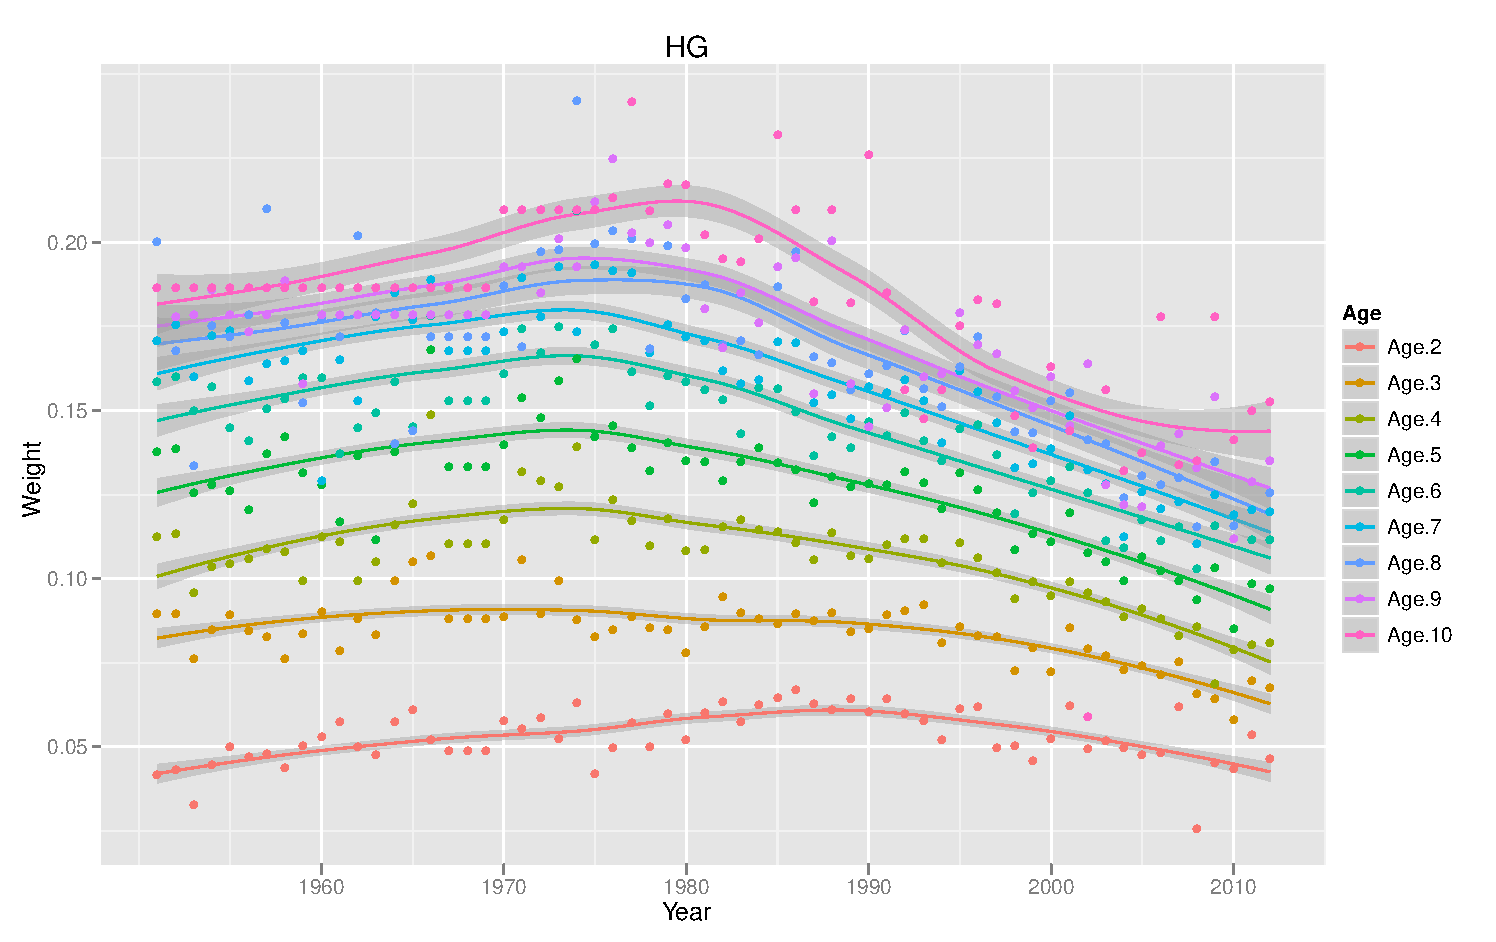
\includegraphics[scale=0.4]
		{../FIGS/iscam_fig_weight-at-age_HG}
		\caption{Haida Gwaii: empirical weight-at-age (kg).}
	\end{figure}
	}
	%
	\only<2>{
	\begin{figure}[htbp]
		\centering
		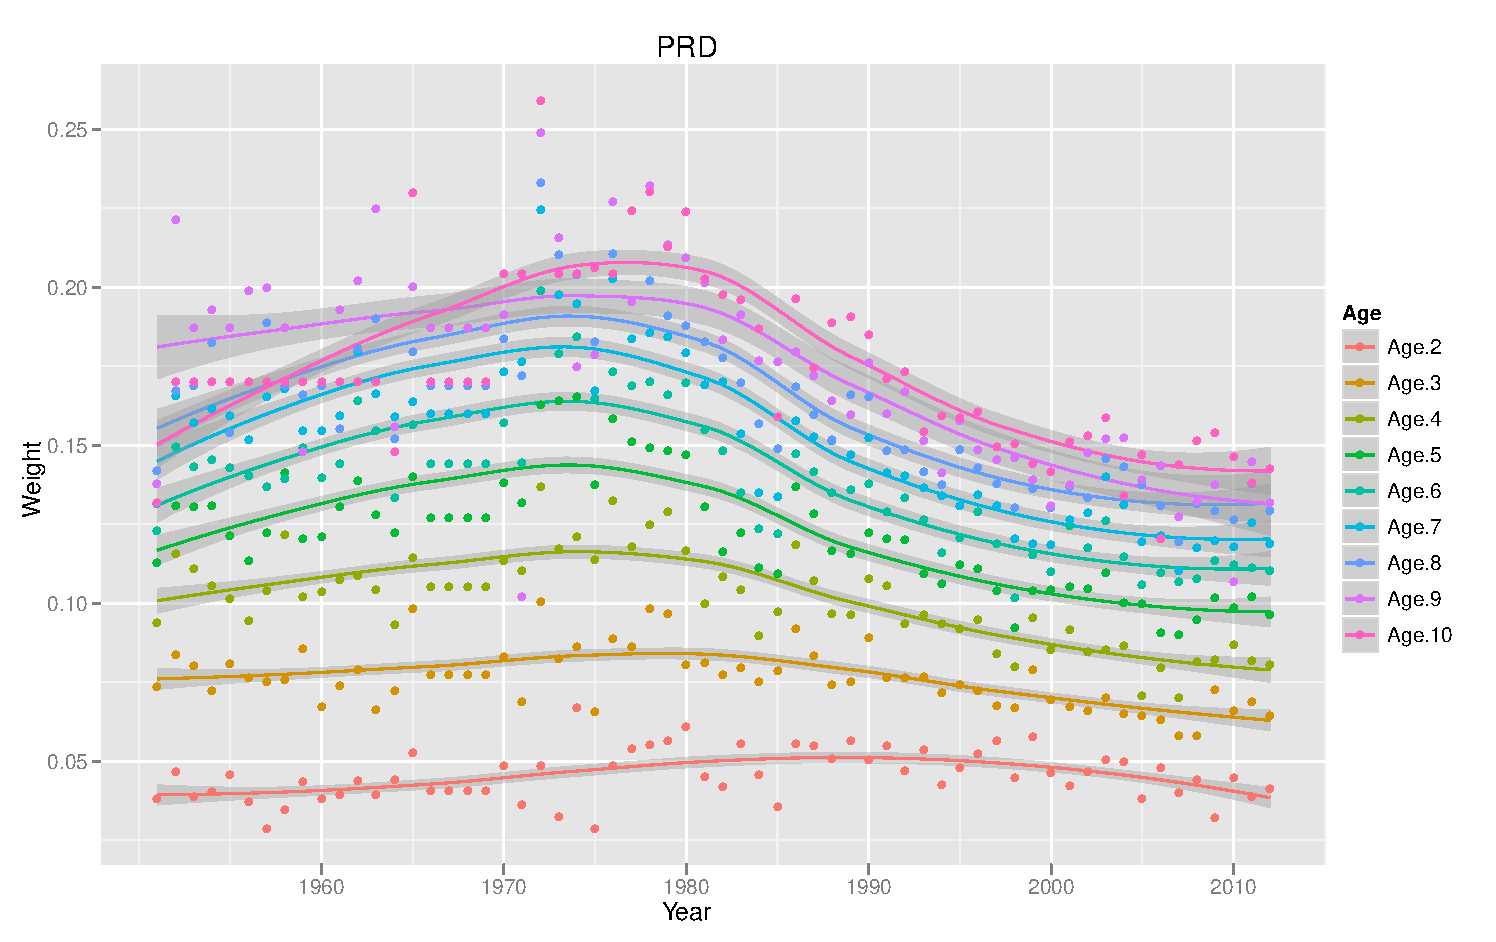
\includegraphics[scale=0.4]
		{../FIGS/iscam_fig_weight-at-age_PRD}
		\caption{Prince Rupert District: empirical weight-at-age (kg).}
	\end{figure}
	}
	%
	\only<3>{
	\begin{figure}[htbp]
		\centering
		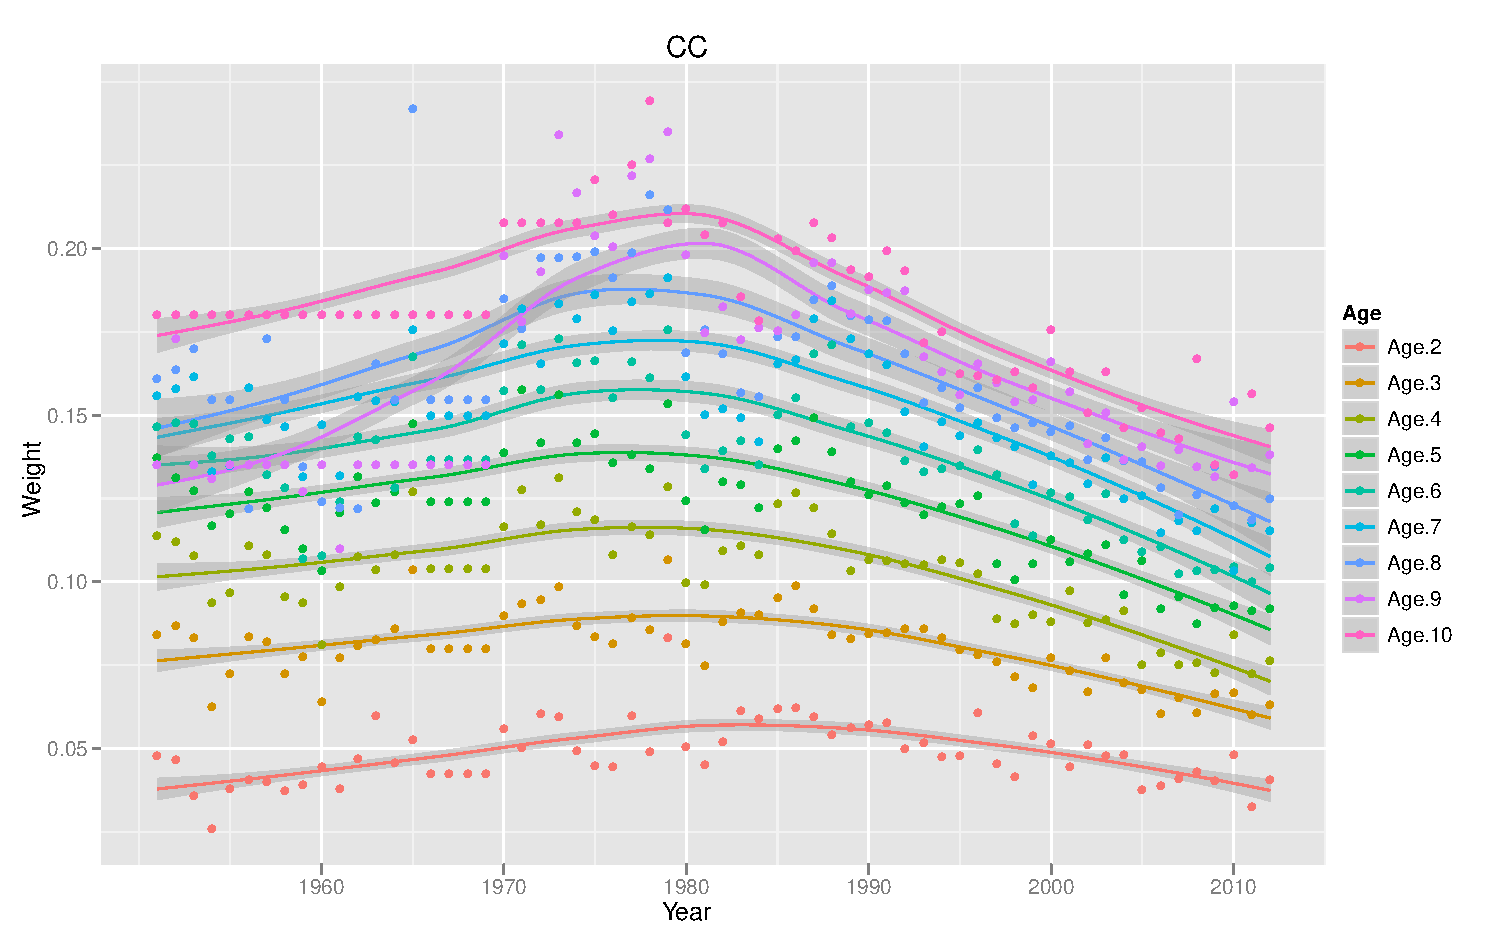
\includegraphics[scale=0.4]
		{../FIGS/iscam_fig_weight-at-age_CC}
		\caption{Central Coast: empirical weight-at-age (kg).}
	\end{figure}
	}
	%
	\only<4>{
	\begin{figure}[htbp]
		\centering
		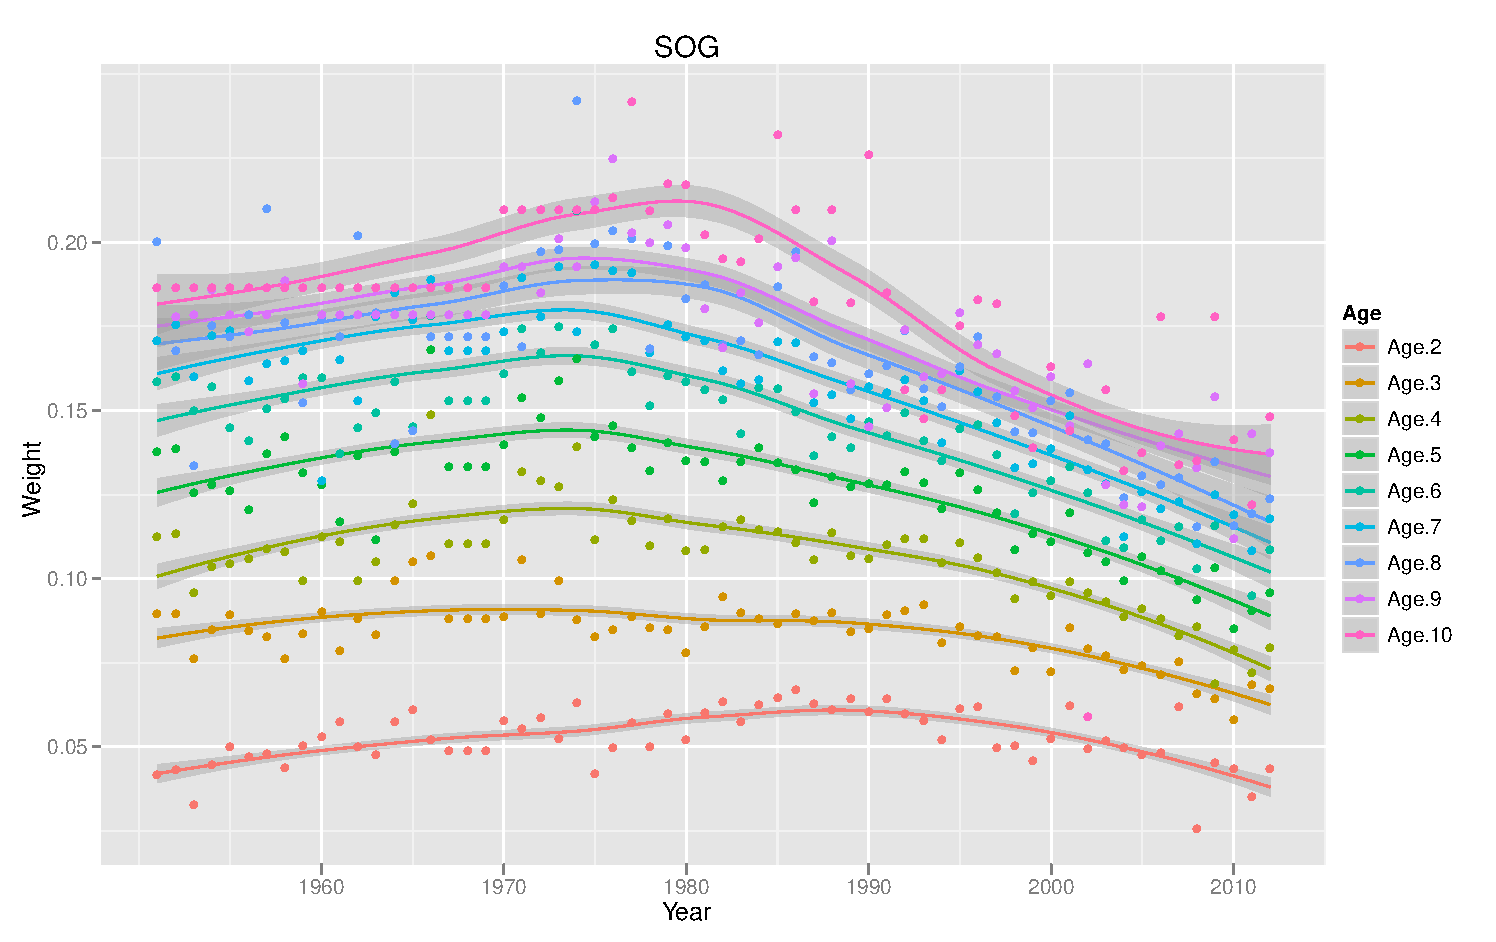
\includegraphics[scale=0.4]
		{../FIGS/iscam_fig_weight-at-age_SOG}
		\caption{Strait of Georgia: empirical weight-at-age (kg).}
	\end{figure}
	}
	%
	\only<5>{
	\begin{figure}[htbp]
		\centering
		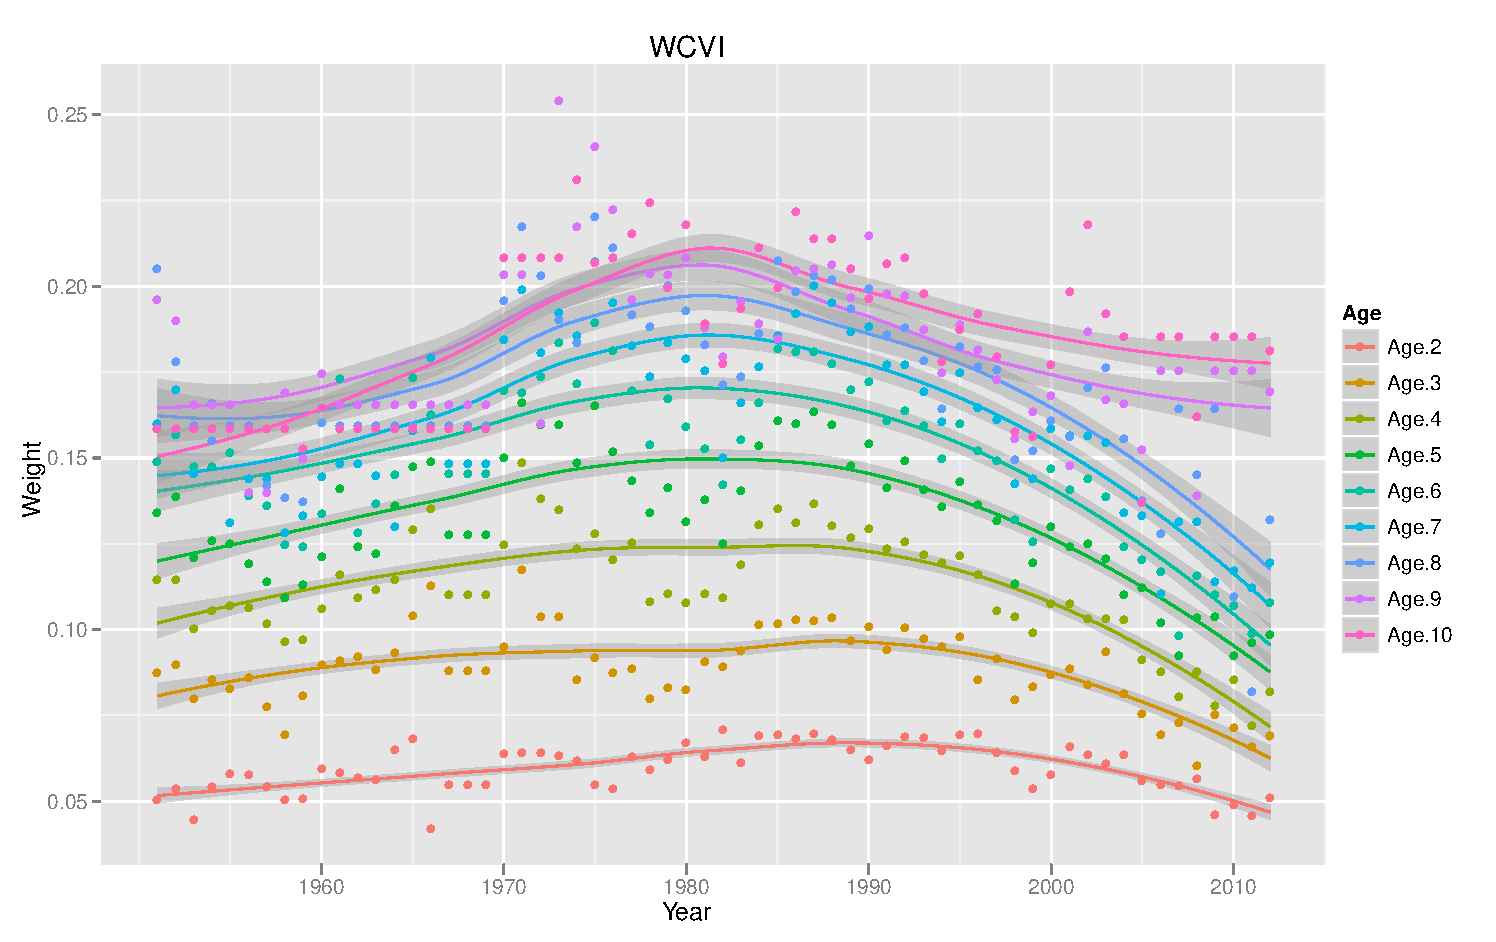
\includegraphics[scale=0.4]
		{../FIGS/iscam_fig_weight-at-age_WCVI}
		\caption{West Coast Vancouver Island: empirical weight-at-age (kg).}
	\end{figure}
	}
	%
\end{frame}
%
% subsection 2011_data (end)

\subsection{Analytical Methods} % (fold)
\label{sub:analytical_methods}
\begin{frame}[t]\frametitle{Analytics \& assumptions}
	\begin{itemize}
		\item<+-> All major and minor areas were assessed using  \iscam.
		\item<+-> Reported catch: CV = 0.005
		\item<+-> Spawn survey: proportional \& 100\% of $Z_t$.
		\item<+-> Dive survey more precise than surface survey.
		\item<+-> Fecundity $\propto$ mature weight-at-age.
		\item<+-> Seine gears: selectivity is asymptotic and time-invariant. 
		\item<+-|alert@+> Gillnet gear: logistic selectivity with weigth-at-age covariates.
		\item<+-|alert@+> $P(\ln(q_1),\ln(q_2)) \sim $ Normal($\mu=-0.569,\sigma=0.274$).
		\item<+-> Homogenous errors in age-composition (multivariate logistic).
		\item<+-> Age-samples $<$0.02 pooled in adjacent cohort.
	\end{itemize}
\end{frame}

\begin{frame}[c]\frametitle{Diagnostics, Forecasts \& Catch Advice}
	\begin{description}
		\item<+->[Diagnostics] Retrospective analysis (sequential removal of the last 10 years of data).
		\item<+->[Forecasts] One-year projection of 3+ biomass with poor, average, good age-3 recruitment.
		\item<+->[Catch advice] Based on HCR with 20\% harvest rate if above cutoff.
	\end{description}
\end{frame}
% subsection analytical_methods (end)

\subsection{Maximum Likelihood Estimates} % (fold)
\label{sub:maximum_likelihood_estimates}
%
\begin{frame}[t]\frametitle{MLE: Spawn survey}
	\only<1>{
	\begin{figure}[htbp]
		\centering
		\vspace{-1cm}
		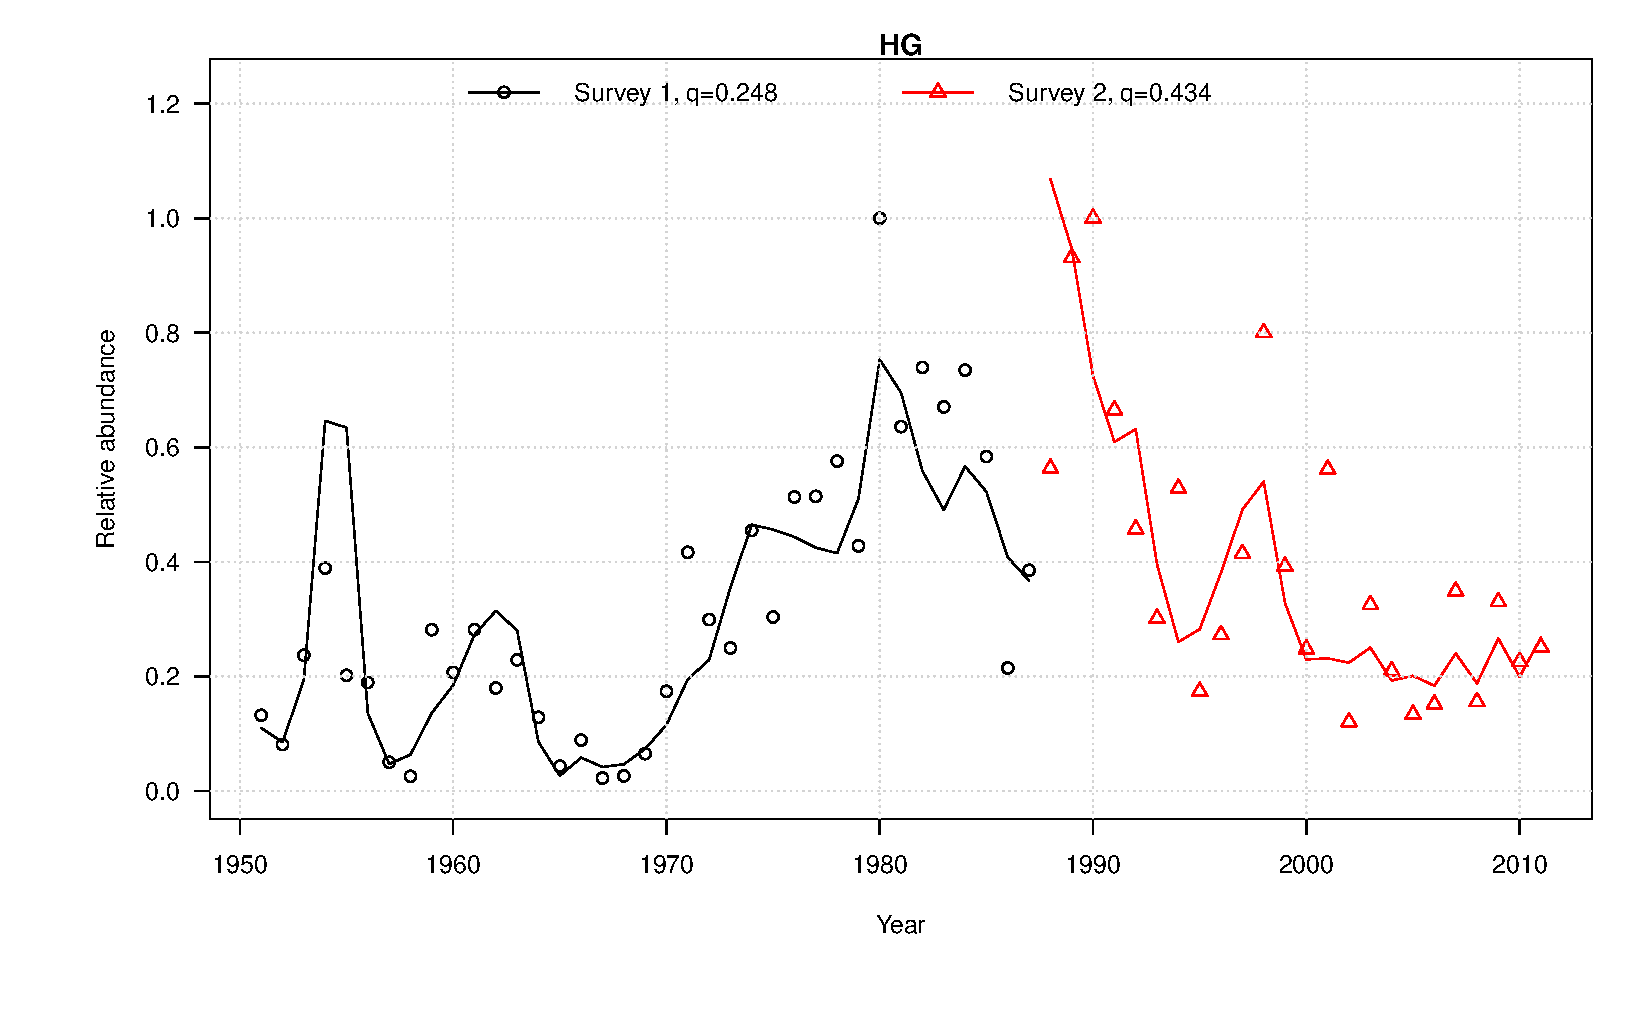
\includegraphics[scale=0.4]
	{../FIGS/qPriorFigs/iscam_fig_survey_fit_HG}
		\vspace{-1cm}
		\caption{Haida Gwaii}
	\end{figure}
	}
	%
	\only<2>{
	\begin{figure}[htbp]
		\centering
		\vspace{-1cm}
		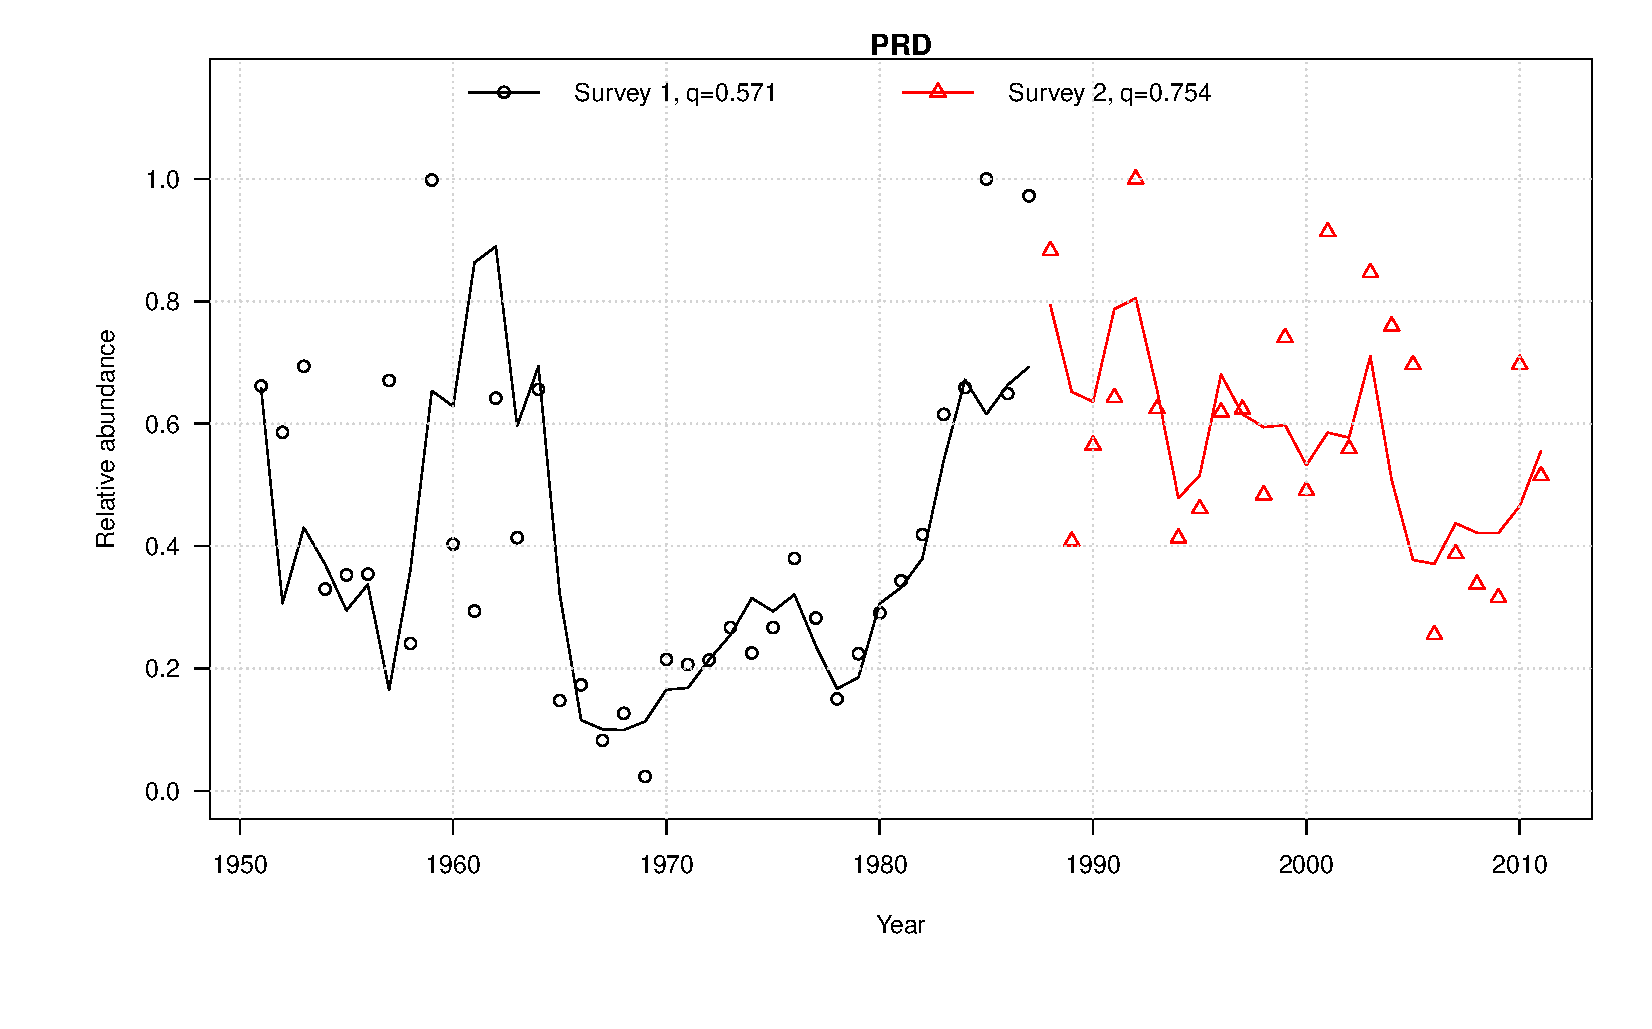
\includegraphics[scale=0.4]
	{../FIGS/qPriorFigs/iscam_fig_survey_fit_PRD}
		\vspace{-1cm}
		\caption{Prince Rupert District}
	\end{figure}
	}
	%
	\only<3>{
	\begin{figure}[htbp]
		\centering
		\vspace{-1cm}
		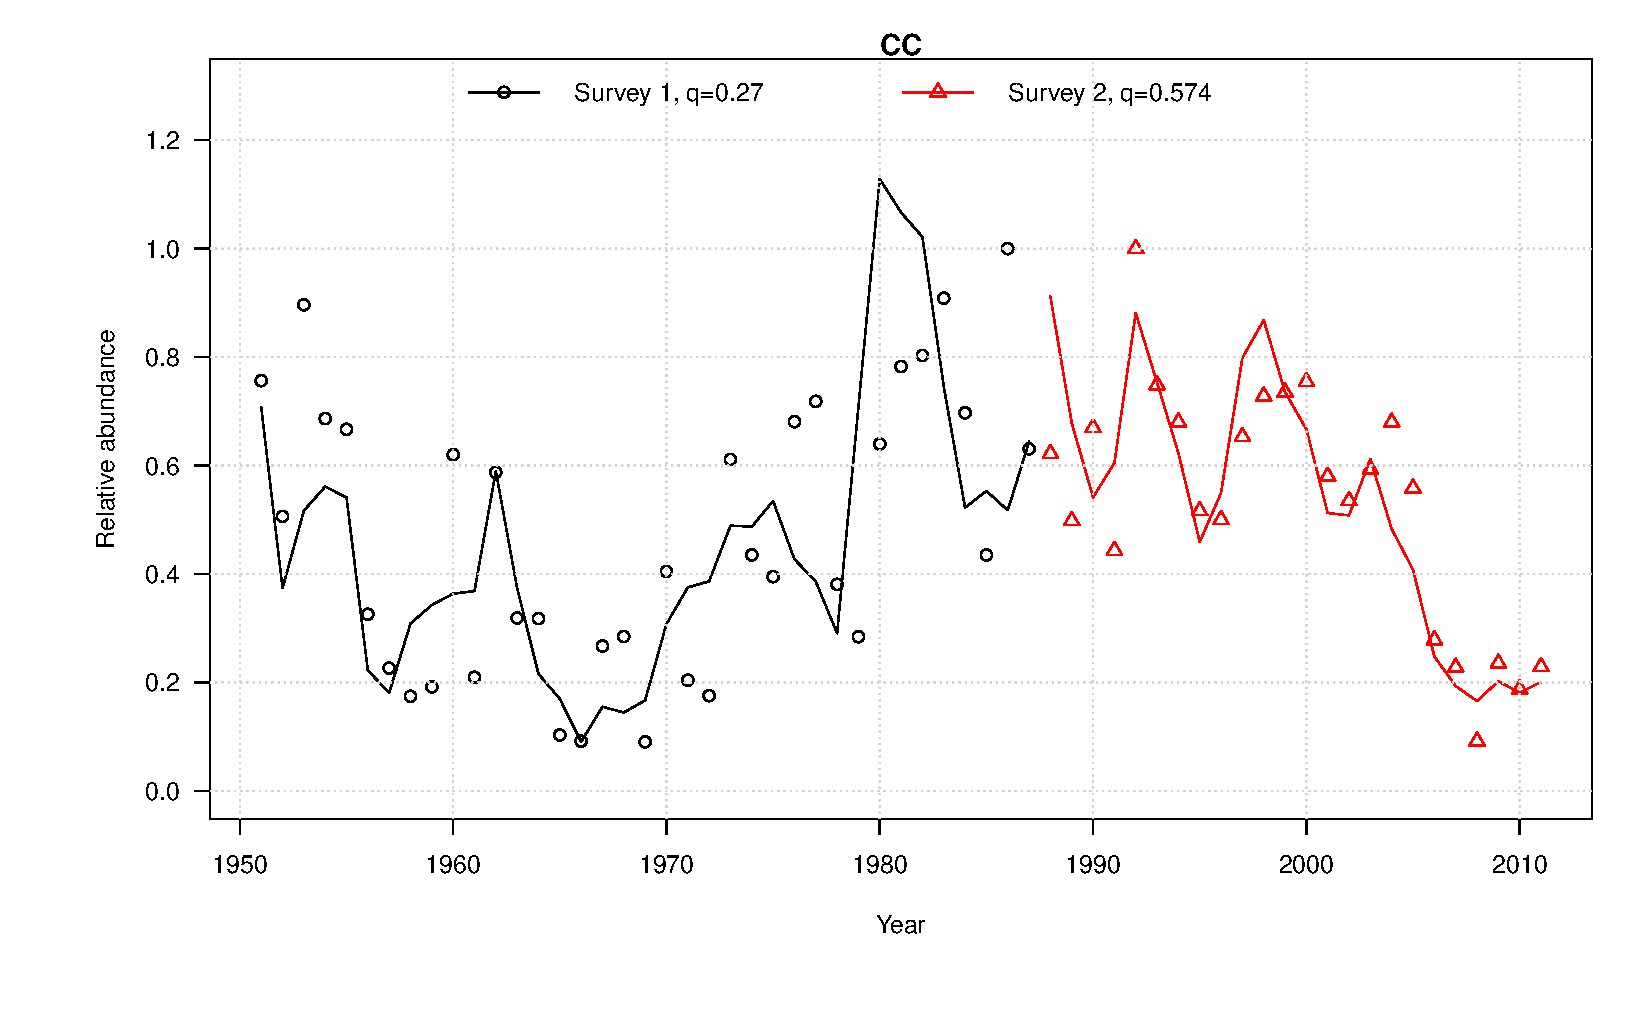
\includegraphics[scale=0.4]
	{../FIGS/qPriorFigs/iscam_fig_survey_fit_CC}
		\vspace{-1cm}
		\caption{Central Coast}
	\end{figure}
	}
	%
	\only<4>{
	\begin{figure}[htbp]
		\centering
		\vspace{-1cm}
		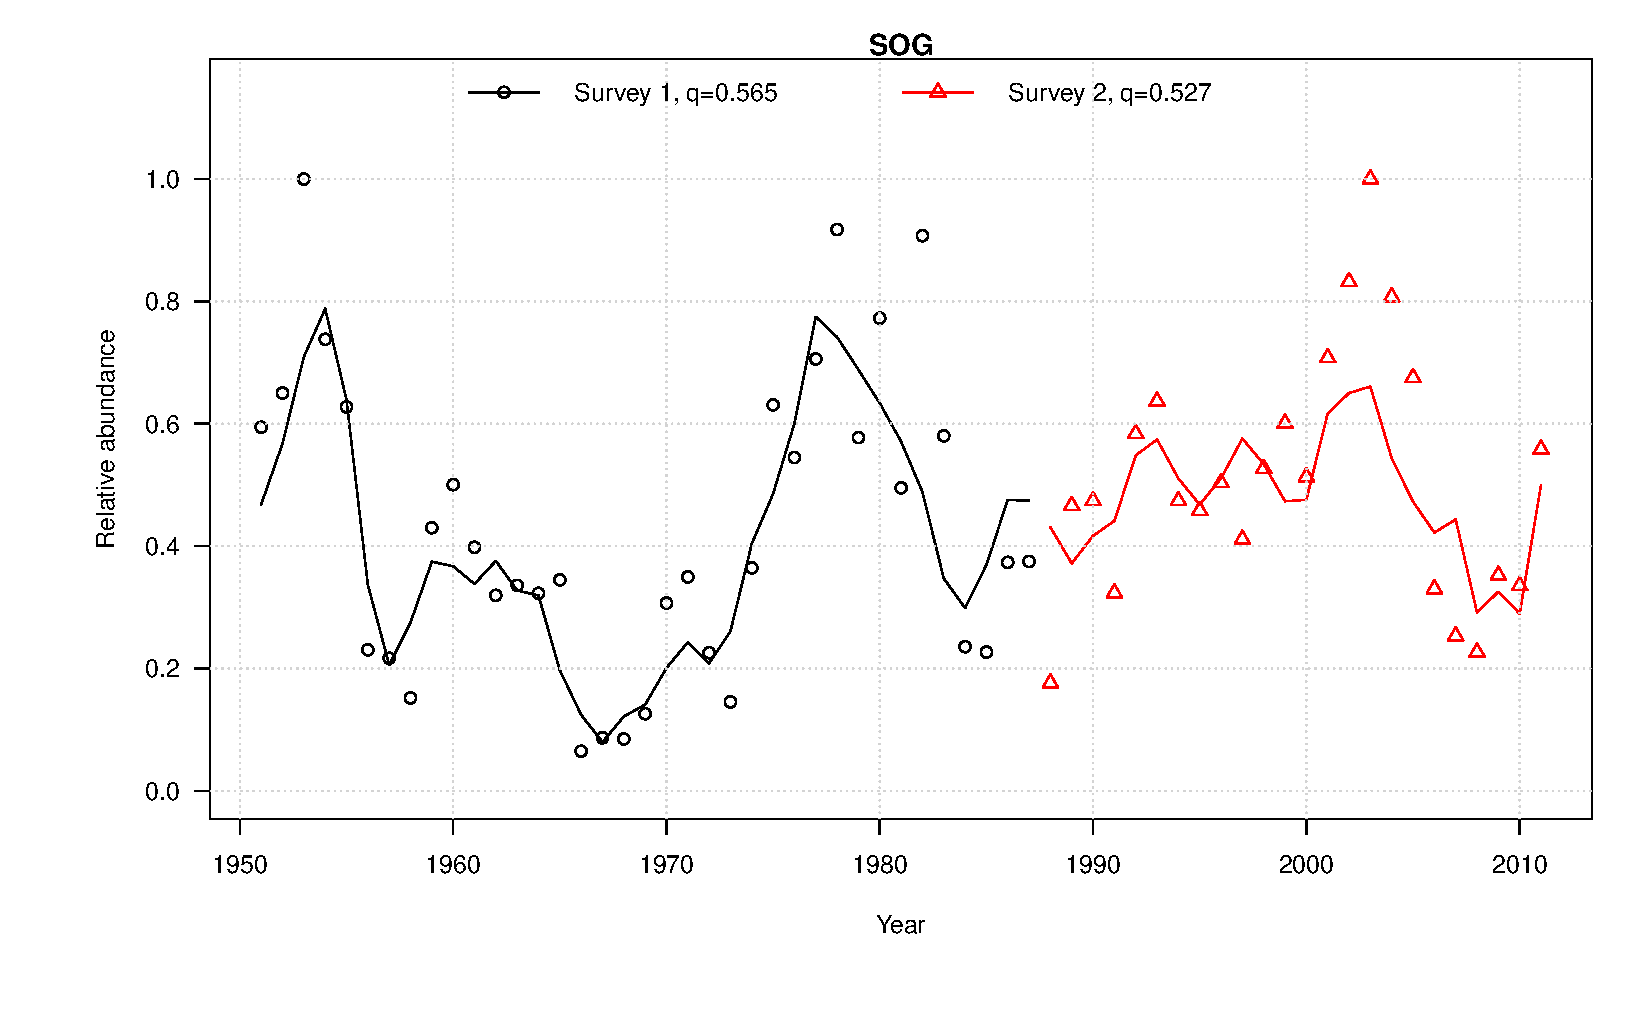
\includegraphics[scale=0.4]
	{../FIGS/qPriorFigs/iscam_fig_survey_fit_SOG}
		\vspace{-1cm}
		\caption{Strait of Georgia}
	\end{figure}
	}
	%
	\only<5>{
	\begin{figure}[htbp]
		\centering
		\vspace{-1cm}
		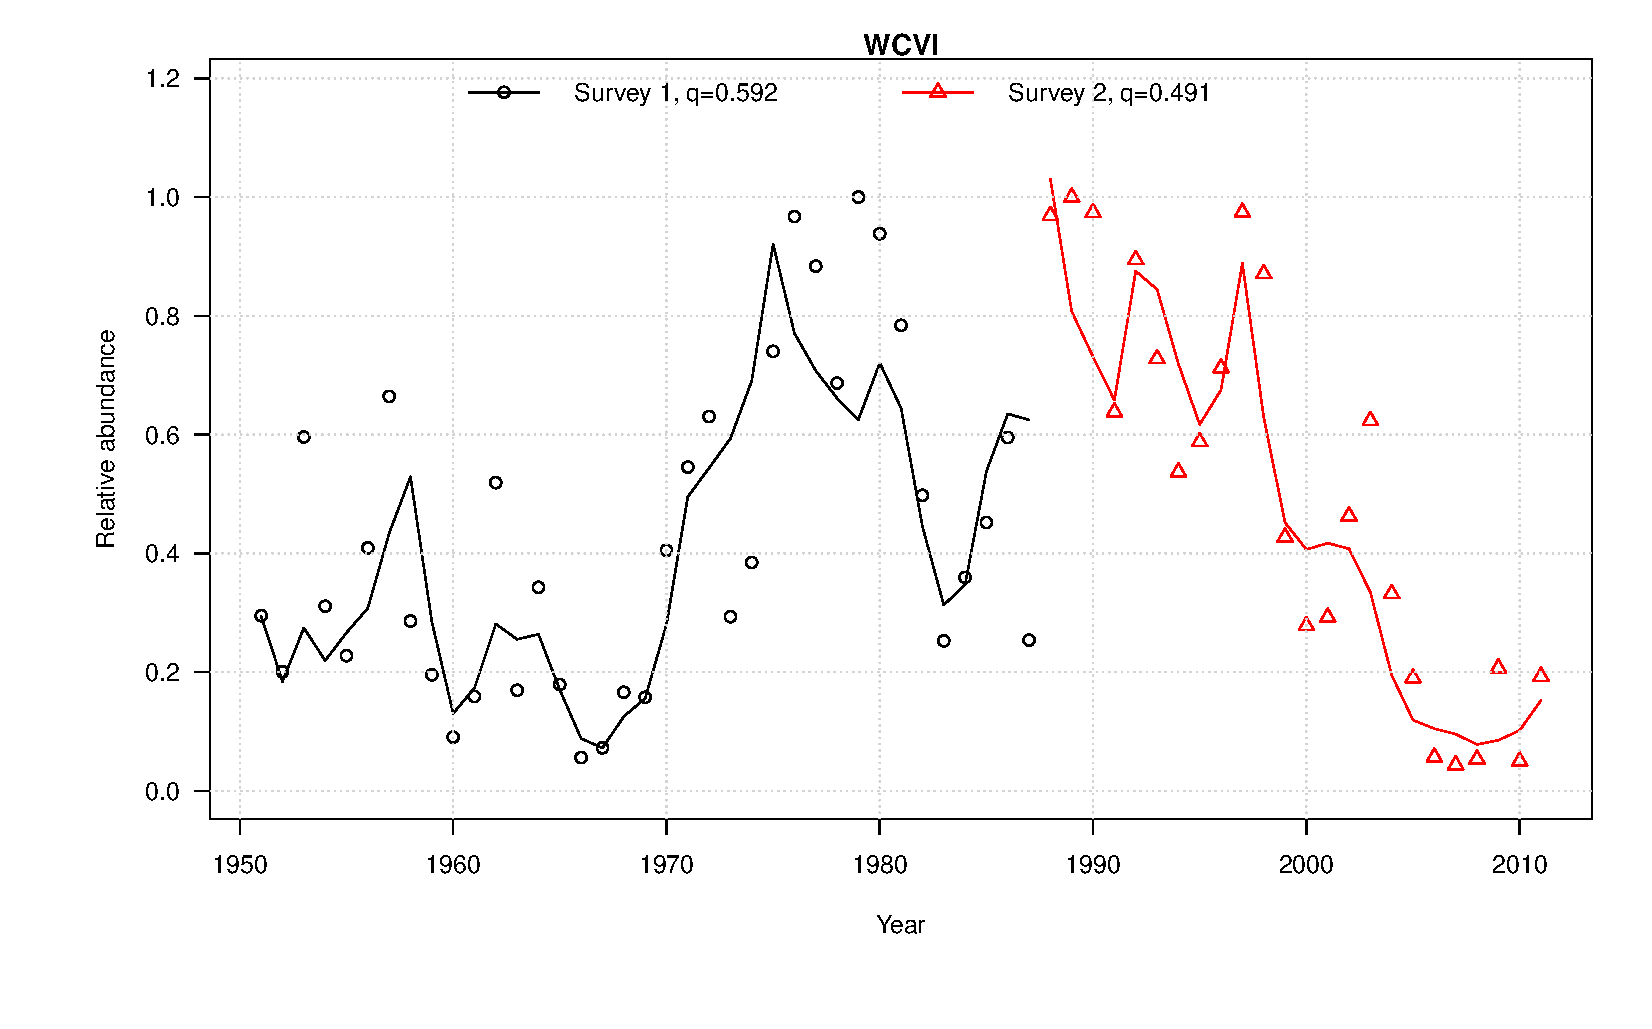
\includegraphics[scale=0.4]
	{../FIGS/qPriorFigs/iscam_fig_survey_fit_WCVI}
		\vspace{-1cm}
		\caption{West Coast Vancouver Island}
	\end{figure}
	}
	%
\end{frame}
%
\begin{frame}[t]\frametitle{MLE: Residuals in age composition data}
	\only<1>{
	\begin{figure}[htbp]
		\centering
		\vspace{-.75cm}
		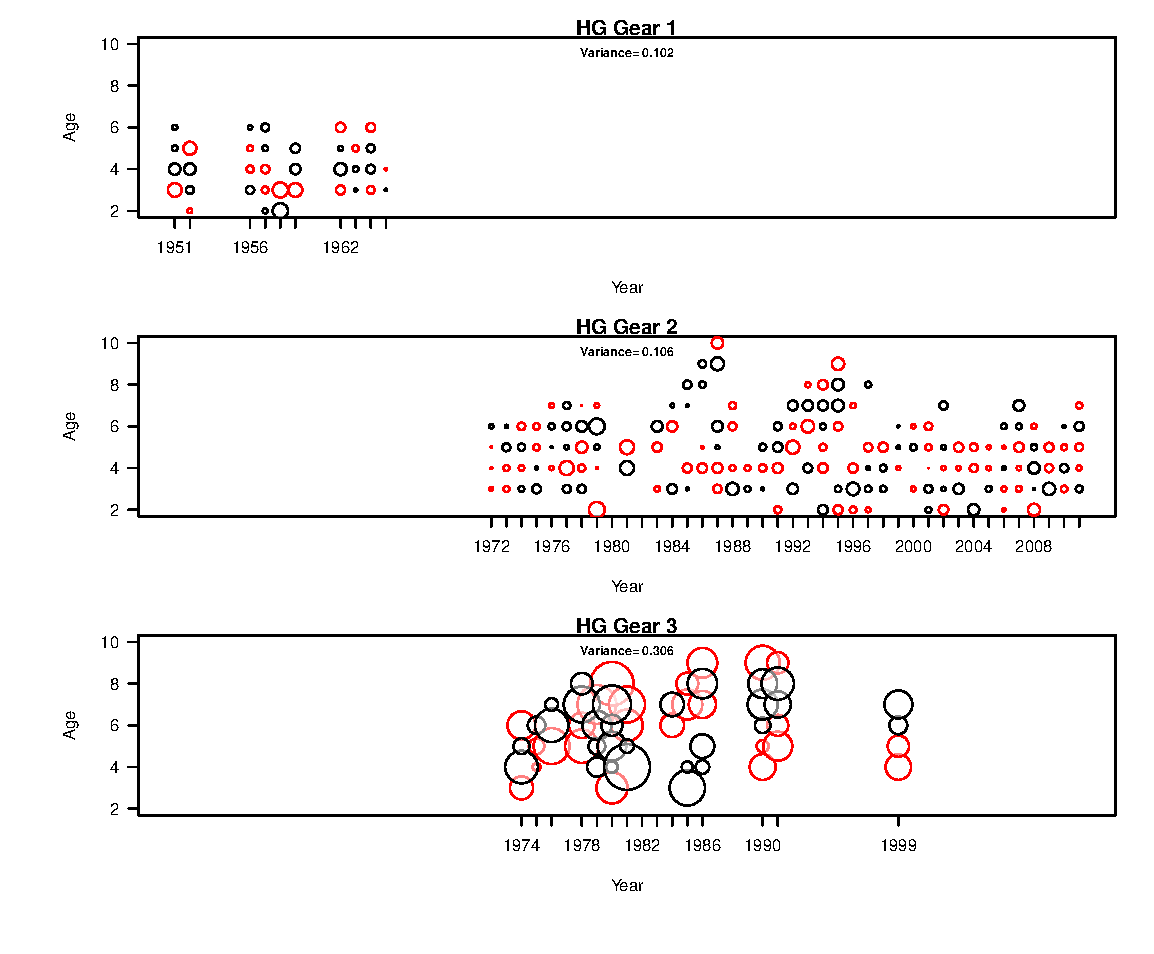
\includegraphics[scale=0.5]
	{../FIGS/qPriorFigs/iscam_fig_agecompsresid_HG}
		\vspace{-1cm}
		\caption{Haida Gwaii}
	\end{figure}
	}
	%
	\only<2>{
	\begin{figure}[htbp]
		\centering
		\vspace{-.75cm}
		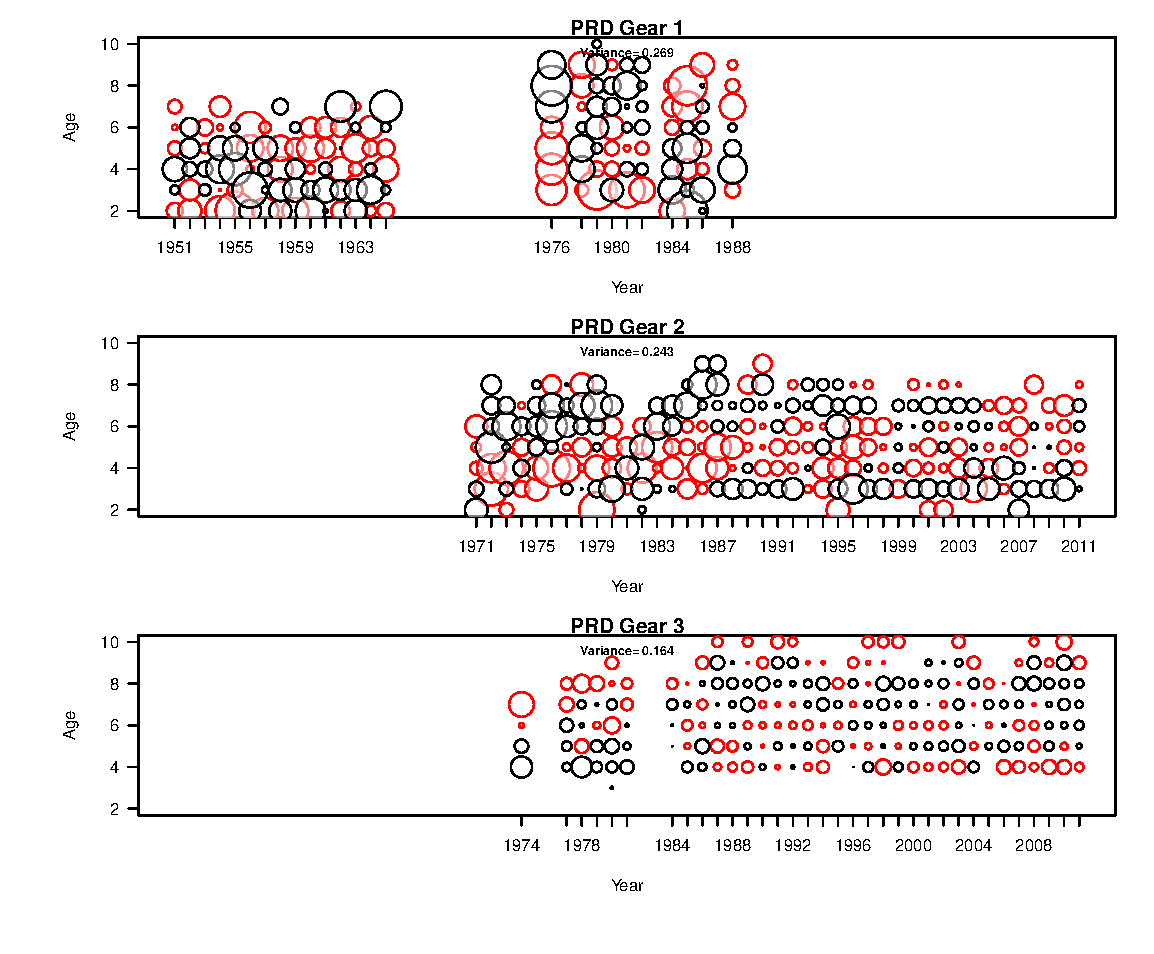
\includegraphics[scale=0.5]
	{../FIGS/qPriorFigs/iscam_fig_agecompsresid_PRD}
		\vspace{-1cm}
		\caption{Prince Rupert District}
	\end{figure}
	}
	%
	\only<3>{
	\begin{figure}[htbp]
		\centering
		\vspace{-.75cm}
		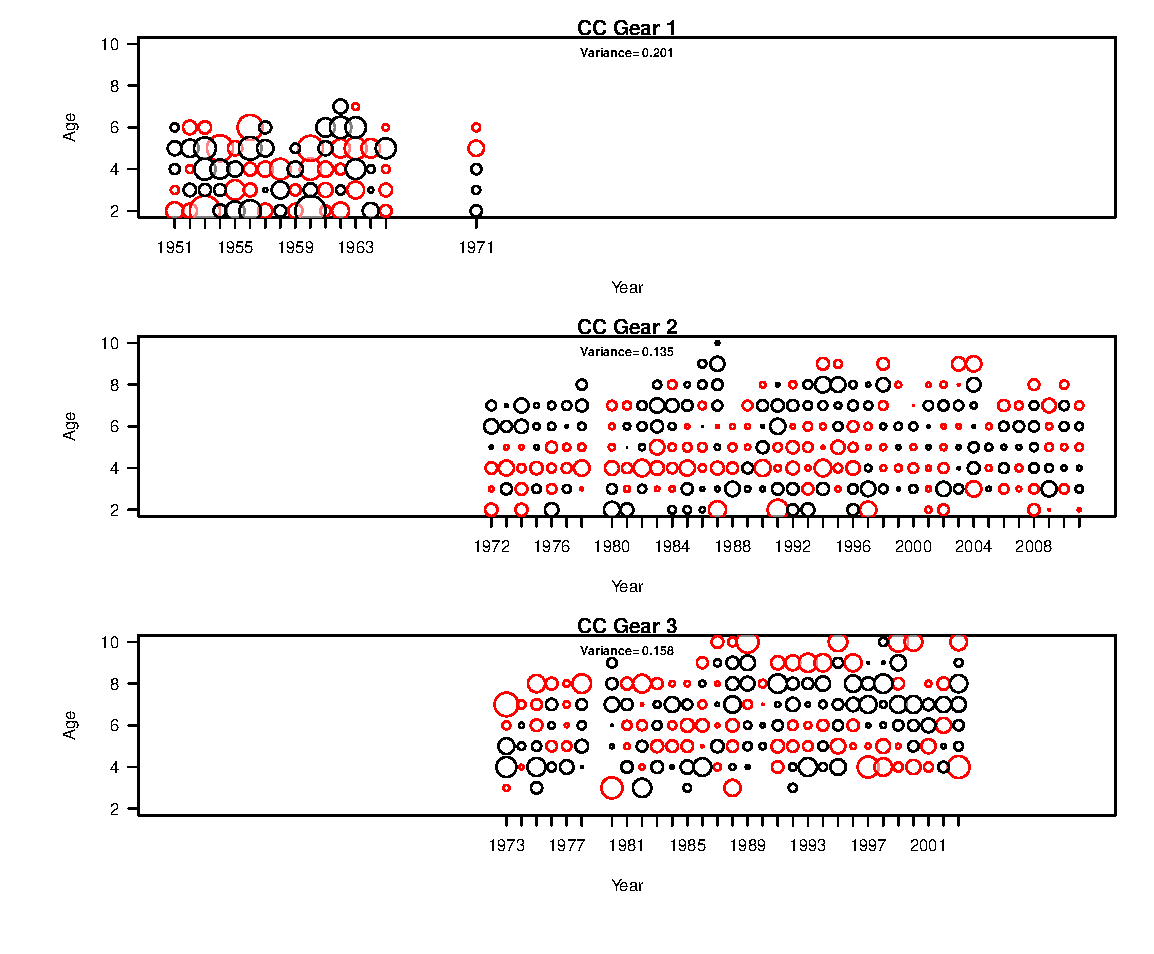
\includegraphics[scale=0.5]
	{../FIGS/qPriorFigs/iscam_fig_agecompsresid_CC}
		\vspace{-1cm}
		\caption{Central Coast}
	\end{figure}
	}
	%
	\only<4>{
	\begin{figure}[htbp]
		\centering
		\vspace{-.75cm}
		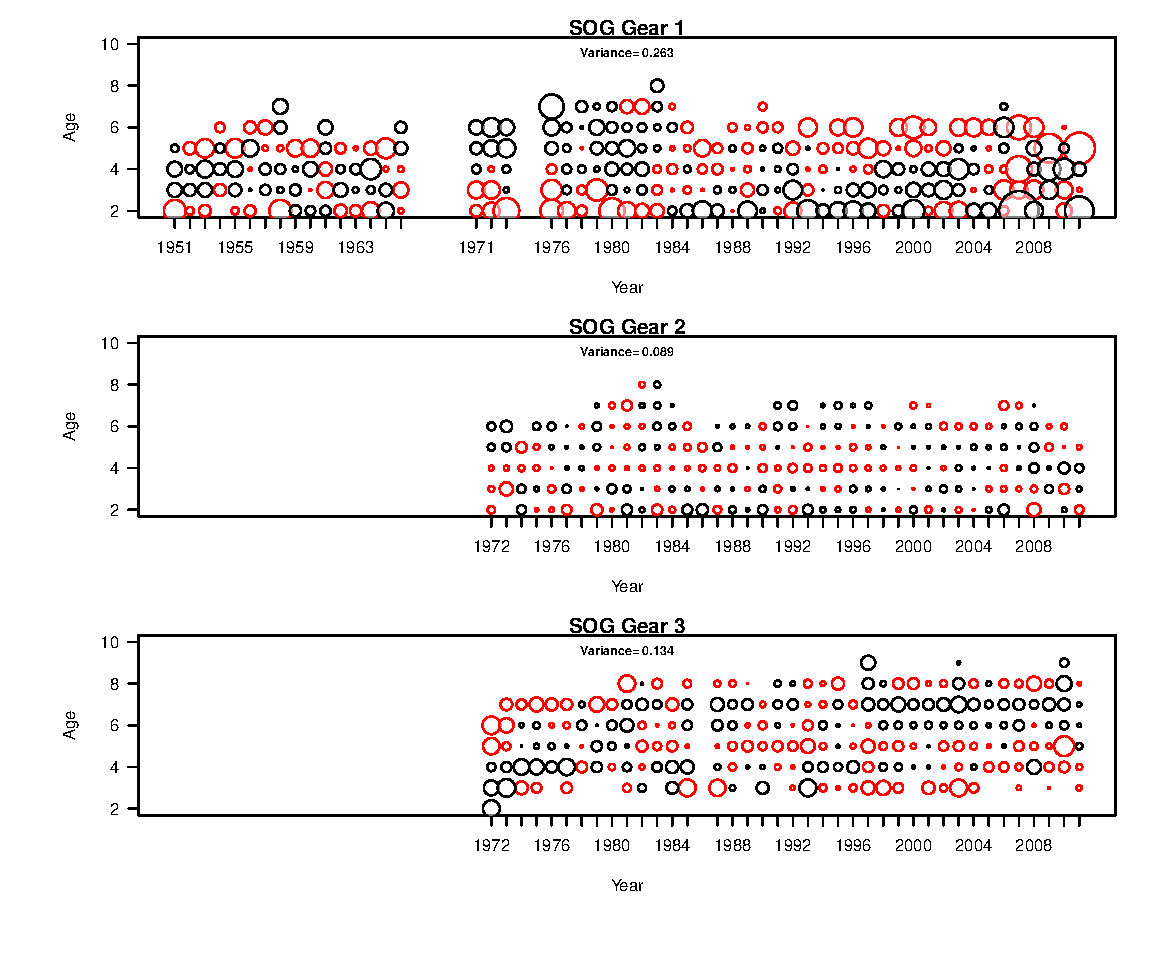
\includegraphics[scale=0.5]
	{../FIGS/qPriorFigs/iscam_fig_agecompsresid_SOG}
		\vspace{-1cm}
		\caption{Strait of Georgia}
	\end{figure}
	}
	%
	\only<5>{
	\begin{figure}[htbp]
		\centering
		\vspace{-.75cm}
		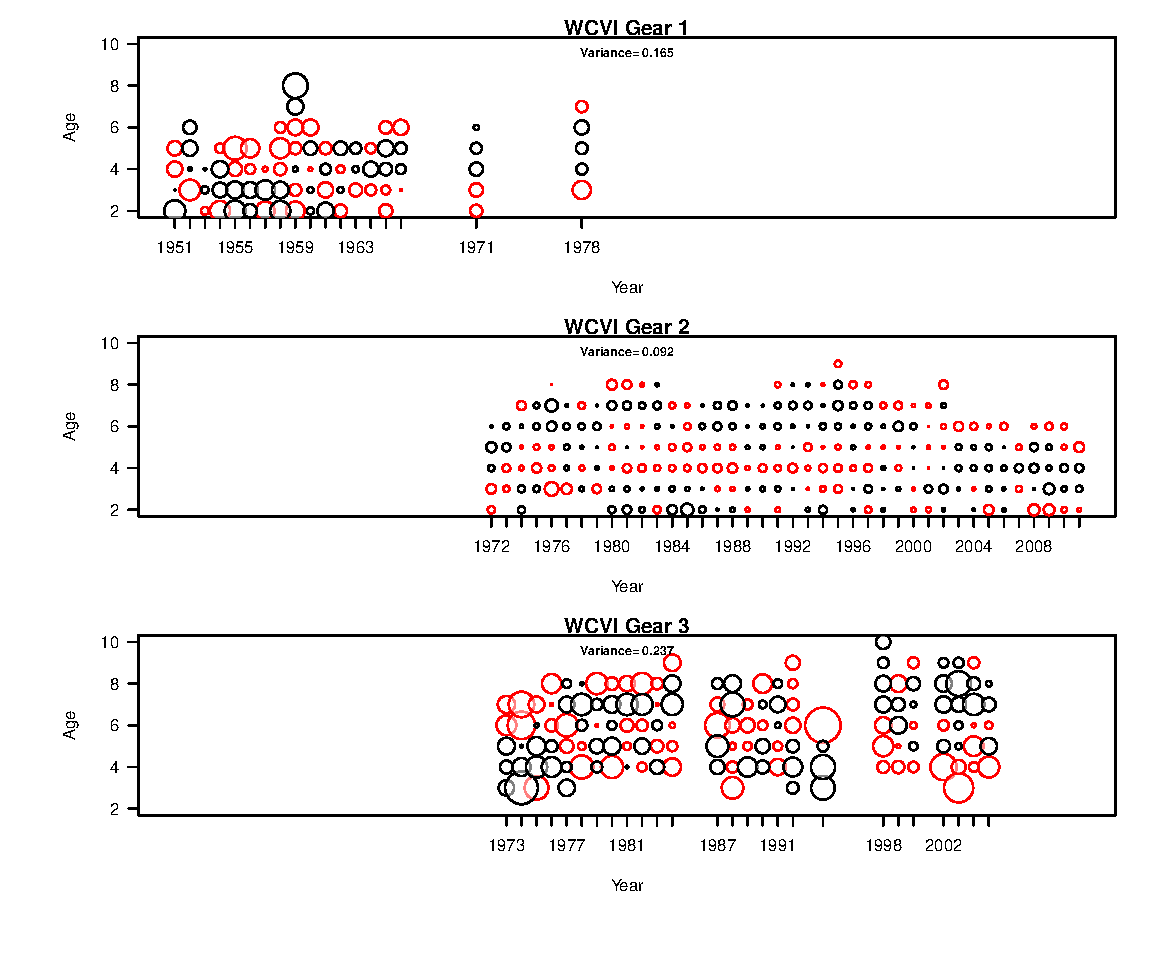
\includegraphics[scale=0.5]
	{../FIGS/qPriorFigs/iscam_fig_agecompsresid_WCVI}
		\vspace{-1cm}
		\caption{West Coast Vancouver Island}
	\end{figure}
	}
	%
\end{frame}
%
\begin{frame}[t]\frametitle{MLE: Mortality}
	\only<1>{
	\begin{figure}[htbp]
		\centering
		\vspace{-1cm}
		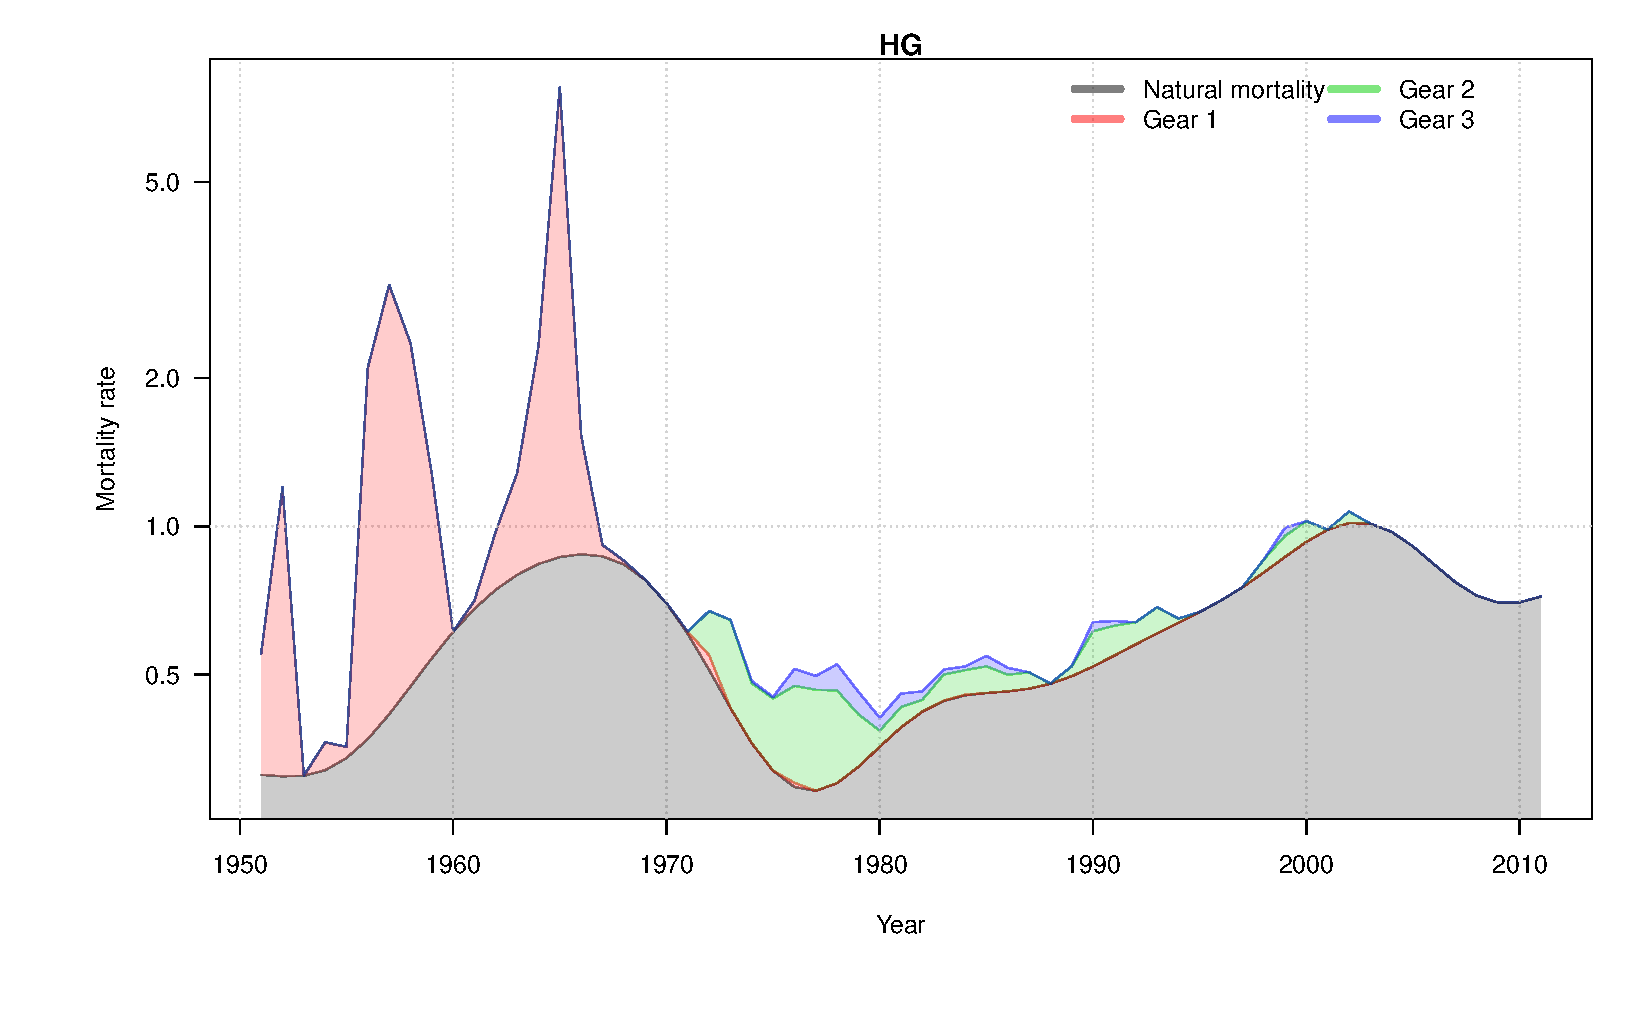
\includegraphics[scale=0.4]
	{../FIGS/qPriorFigs/iscam_fig_mortality_HG}
		\vspace{-1cm}
		\caption{Haida Gwaii}
	\end{figure}
	}
	%
	\only<2>{
	\begin{figure}[htbp]
		\centering
		\vspace{-1cm}
		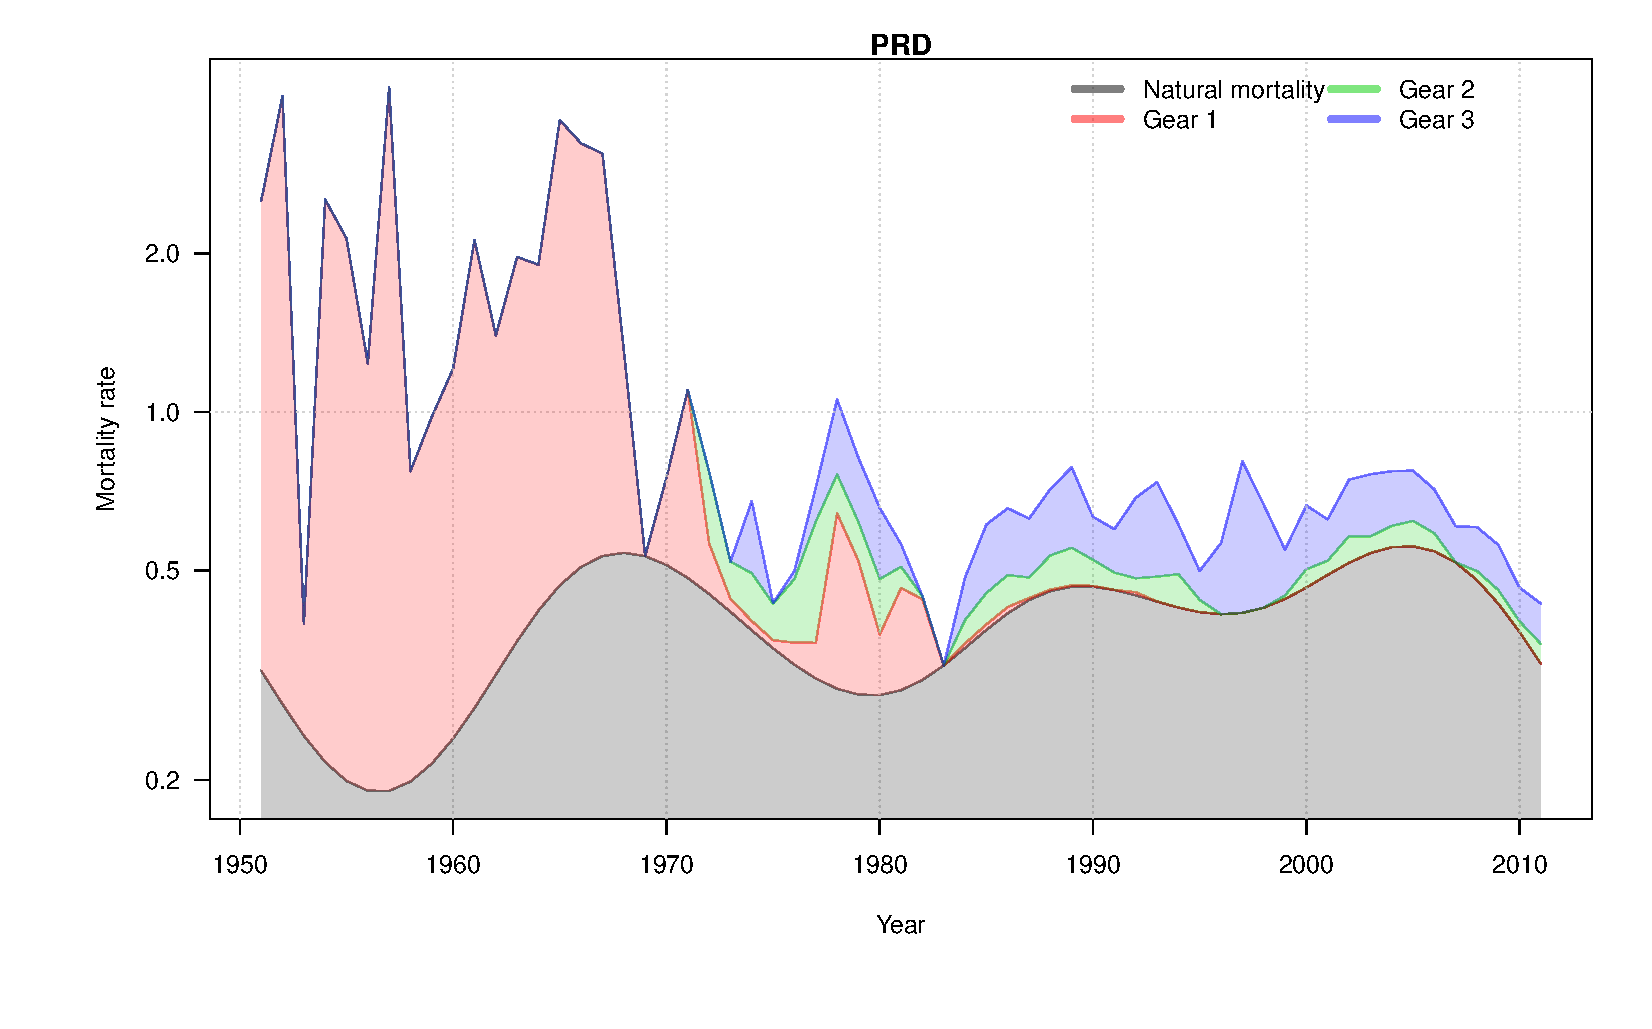
\includegraphics[scale=0.4]
	{../FIGS/qPriorFigs/iscam_fig_mortality_PRD}
		\vspace{-1cm}
		\caption{Prince Rupert District}
	\end{figure}
	}
	%
	\only<3>{
	\begin{figure}[htbp]
		\centering
		\vspace{-1cm}
		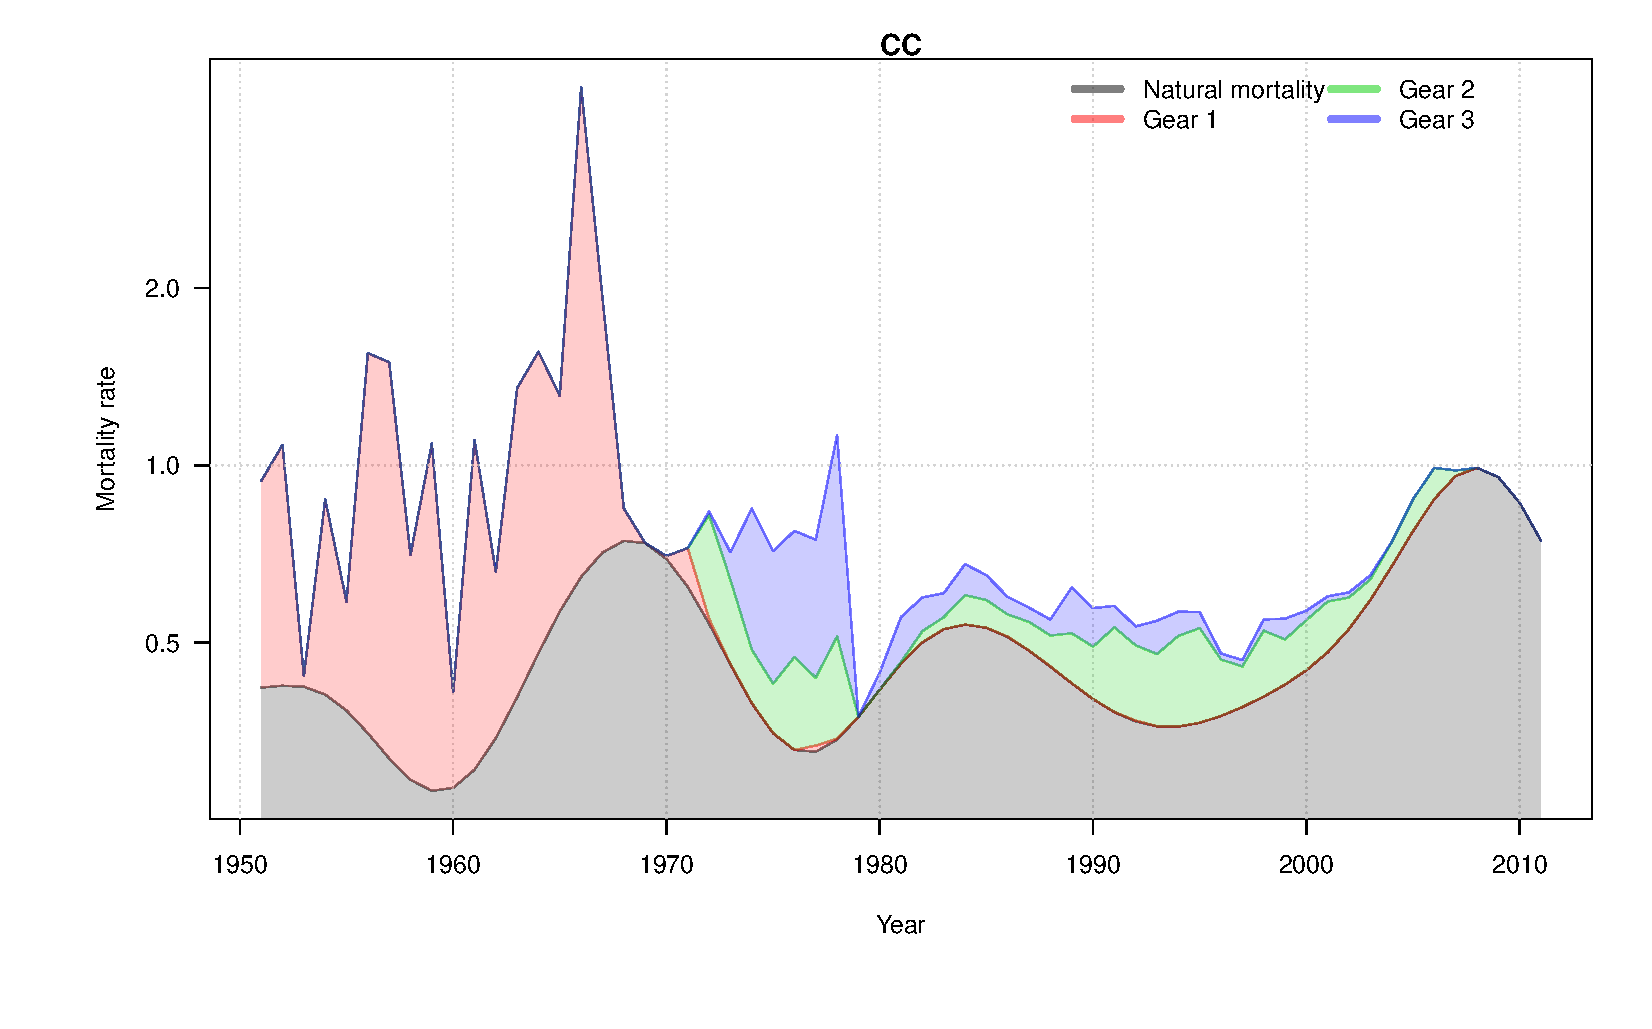
\includegraphics[scale=0.4]
	{../FIGS/qPriorFigs/iscam_fig_mortality_CC}
		\vspace{-1cm}
		\caption{Central Coast}
	\end{figure}
	}
	%
	\only<4>{
	\begin{figure}[htbp]
		\centering
		\vspace{-1cm}
		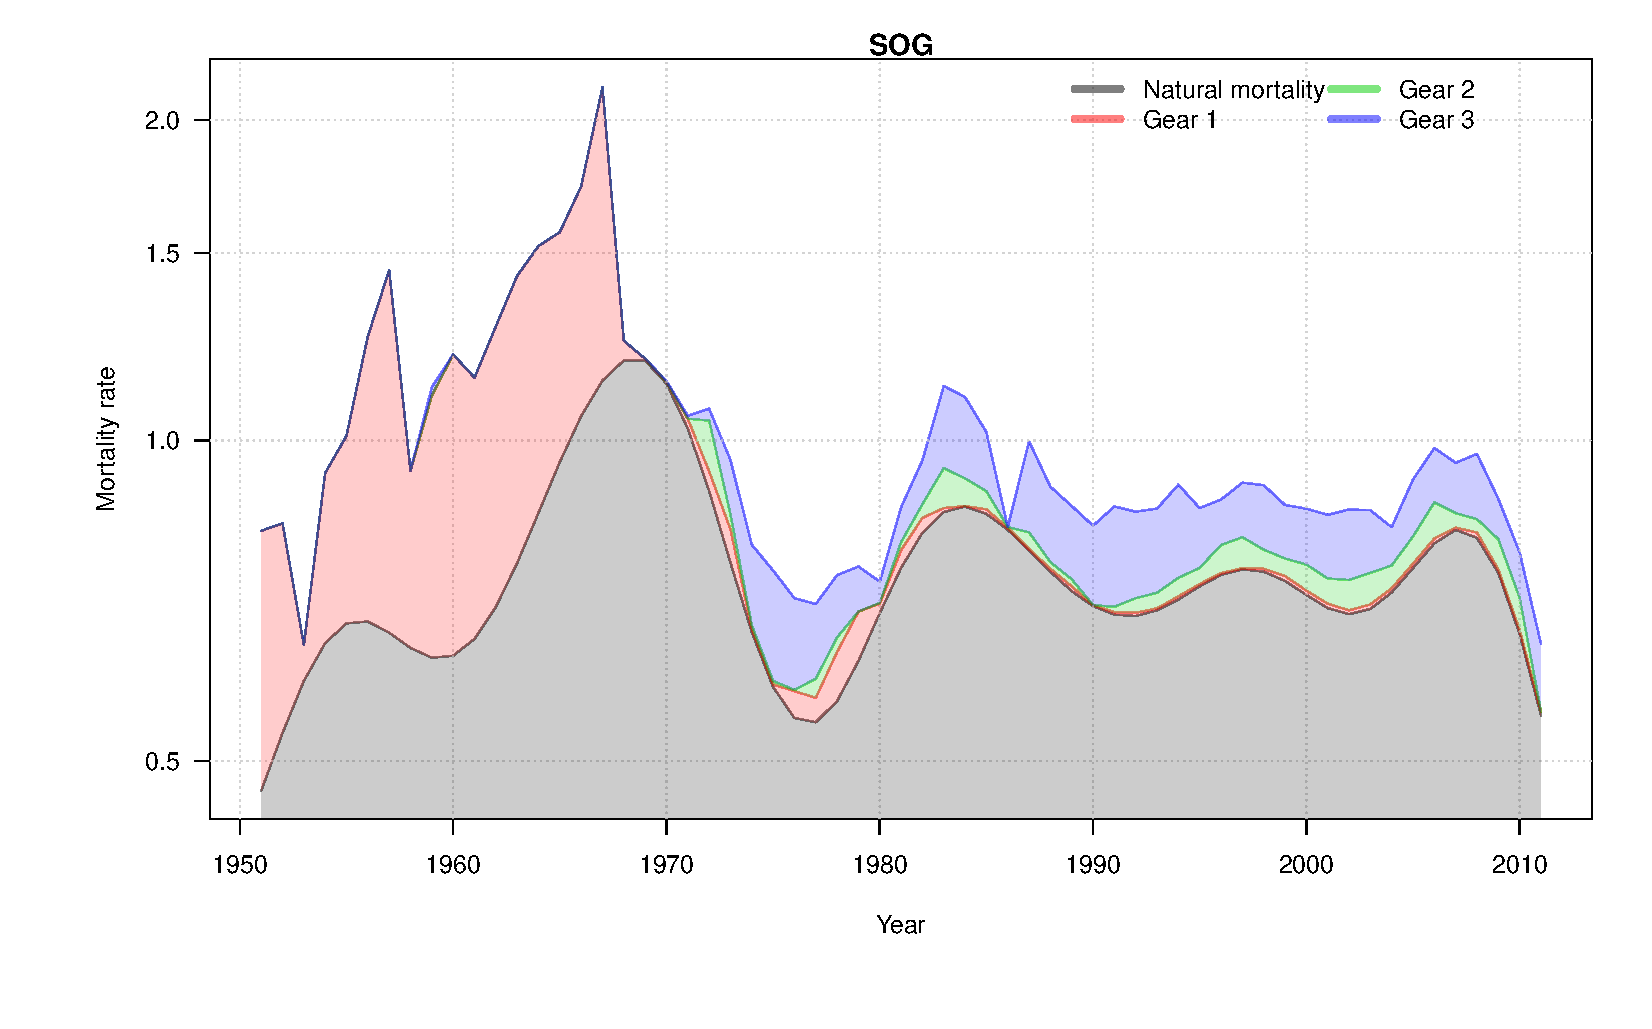
\includegraphics[scale=0.4]
	{../FIGS/qPriorFigs/iscam_fig_mortality_SOG}
		\vspace{-1cm}
		\caption{Strait of Georgia}
	\end{figure}
	}
	%
	\only<5>{
	\begin{figure}[htbp]
		\centering
		\vspace{-1cm}
		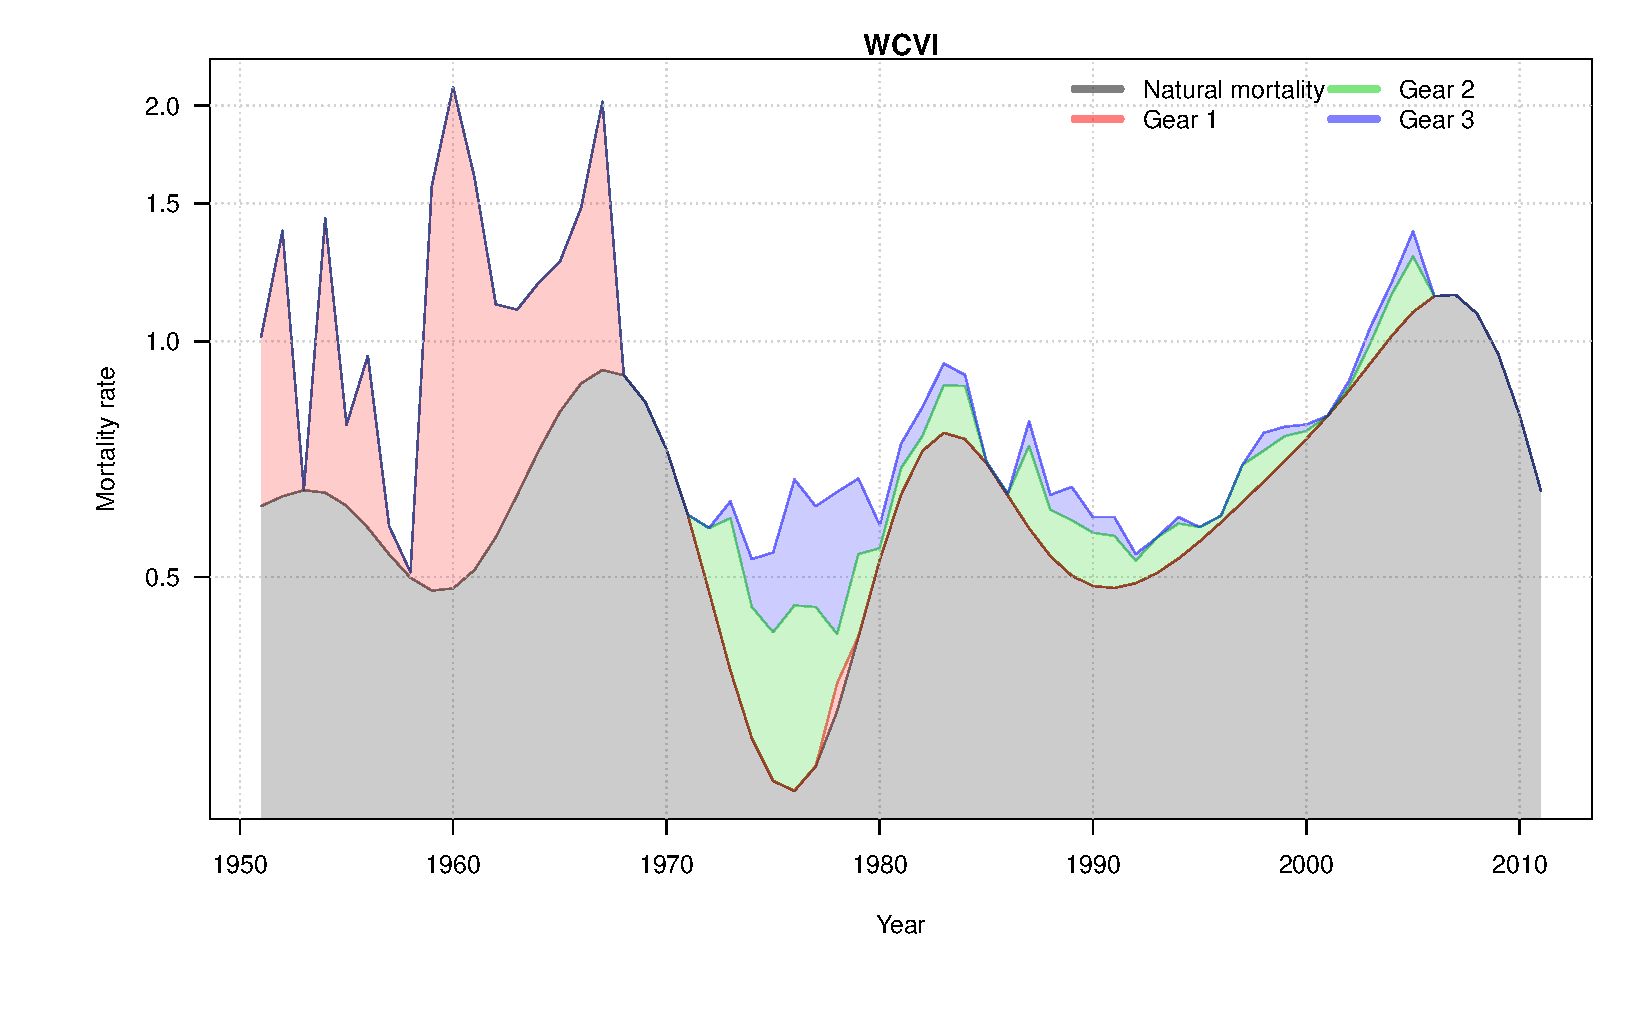
\includegraphics[scale=0.4]
	{../FIGS/qPriorFigs/iscam_fig_mortality_WCVI}
		\vspace{-1cm}
		\caption{West Coast Vancouver Island}
	\end{figure}
	}
	%
\end{frame}
%
\begin{frame}[t]\frametitle{Age-2 recruits}
	\begin{figure}[htbp]
		\centering
		\vspace{-1cm}	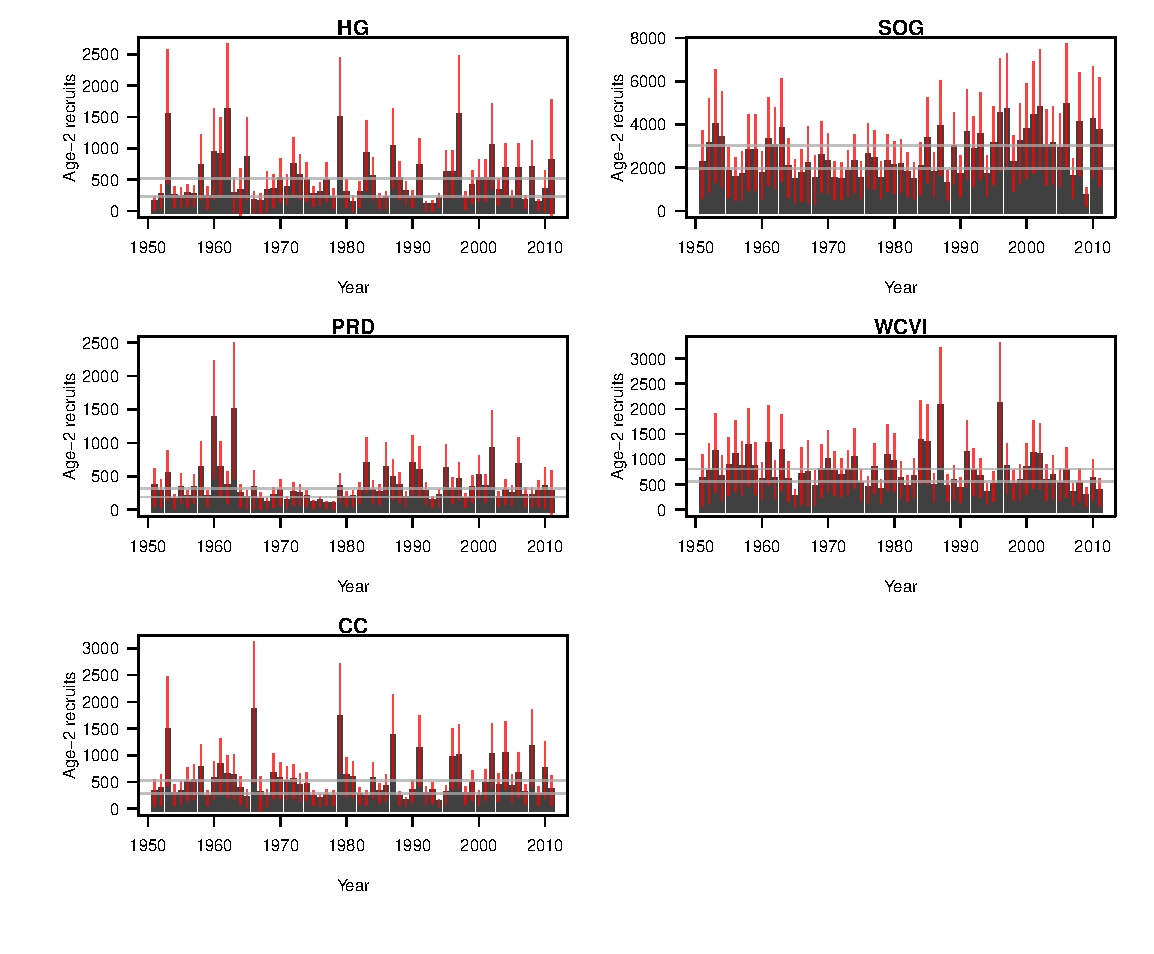
\includegraphics[scale=0.5]{../FIGS/qPriorFigs/iscam_fig_recruitment}
		\vspace{-1cm}
		\caption{Age-2 recruits with 0.33 and 0.66 quantiles.}
	\end{figure}
\end{frame}
%% subsection maximum_likelihood_estimates (end)

\subsection{Diagnostics} % (fold)
\label{sub:diagnostics}
%
\begin{frame}[t]\frametitle{Diagnostics: Retrospective plots}
	\begin{figure}[htbp]
		\centering
		\vspace{-.75cm}	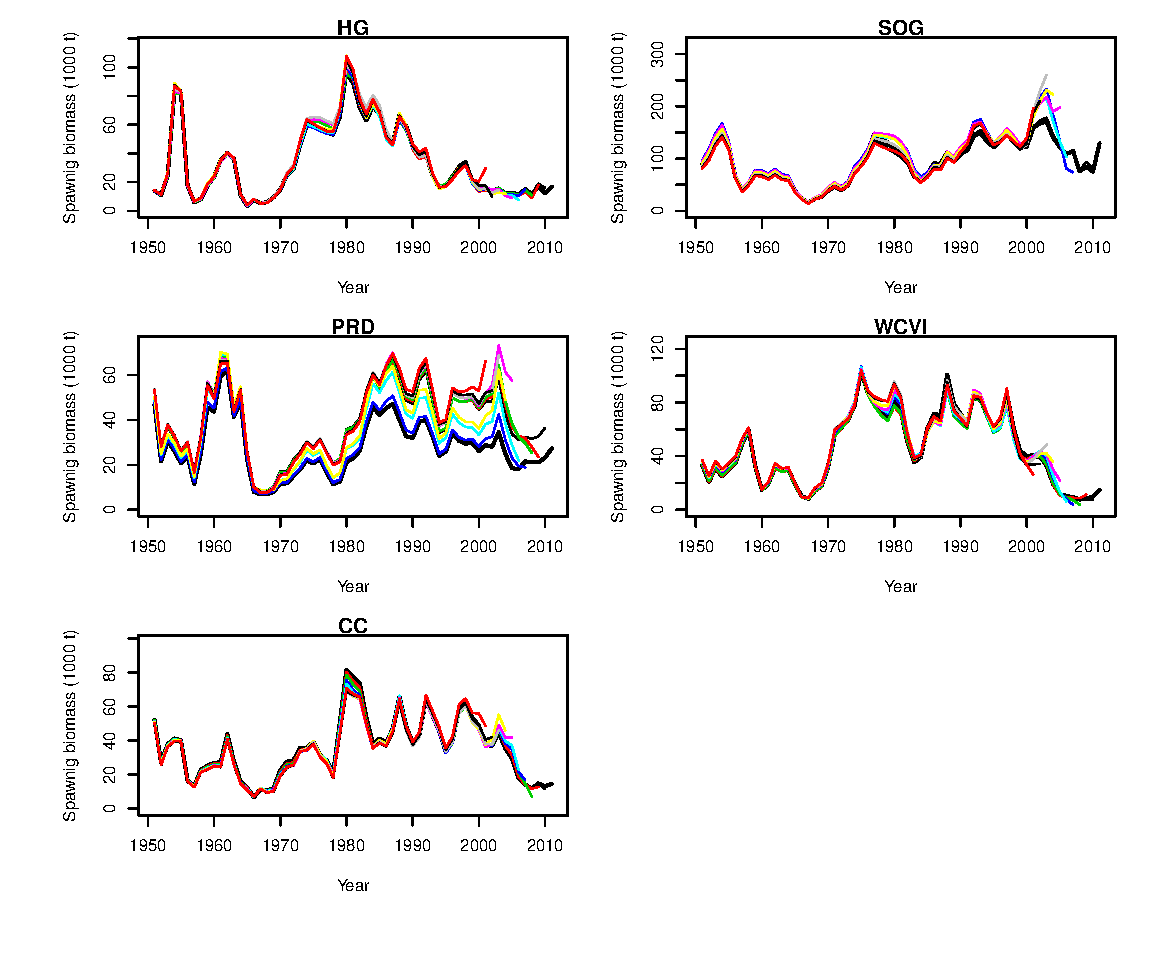
\includegraphics[scale=0.45]{../FIGS/qPriorFigs/iscam_fig_sbt_retrospective}	
		\vspace{-1cm}
		\caption{Retrospective estimates of spawning biomass.}
	\end{figure}
\end{frame}
%
\begin{frame}[t]\frametitle{Diagnostics: Trace plots}
	\begin{figure}[htbp]
		\centering
		\vspace{-0.75cm}	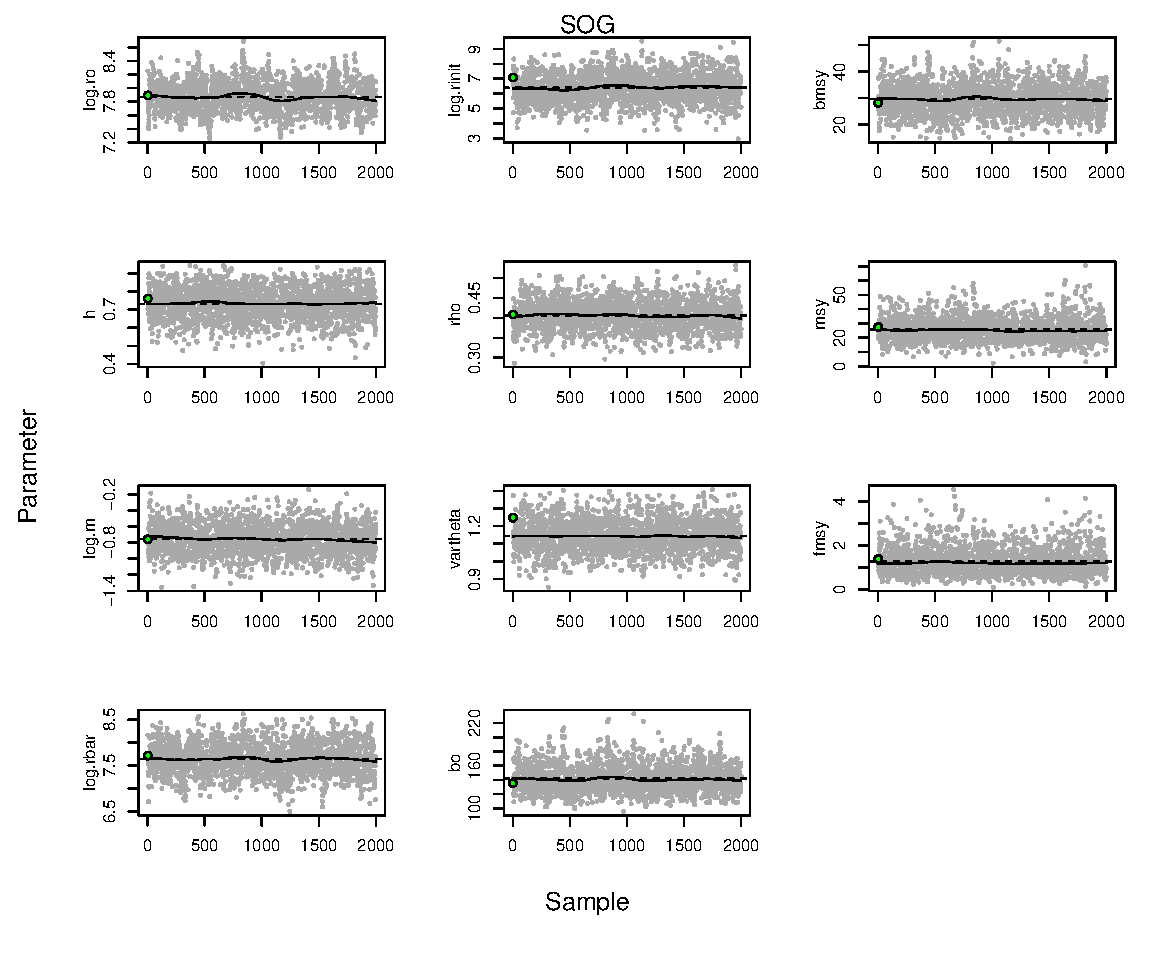
\includegraphics[scale=0.35]{../FIGS/qPriorFigs/iscam_fig_trace_SOG}
		\vspace{-0.65cm}
		\caption{Posterior samples: 1 million, thin 500, Strait of Georgia}
	\end{figure}
	
\end{frame}
%
\begin{frame}[t]\frametitle{Diagnostics: Pair plots}
	\begin{figure}[htbp]
		\centering
		\vspace{-0.75cm}	\includegraphics[scale=0.35]
		{../FIGS/qPriorFigs/iscam_fig_pairs_SOG}
		\vspace{-0.65cm}
		\caption{Posterior samples from leading parameters \& derived variables.}
	\end{figure}
\end{frame}
%
\begin{frame}[t]\frametitle{Diagnositcs: Marginal posteriors}
	\begin{figure}[htbp]
		\centering
			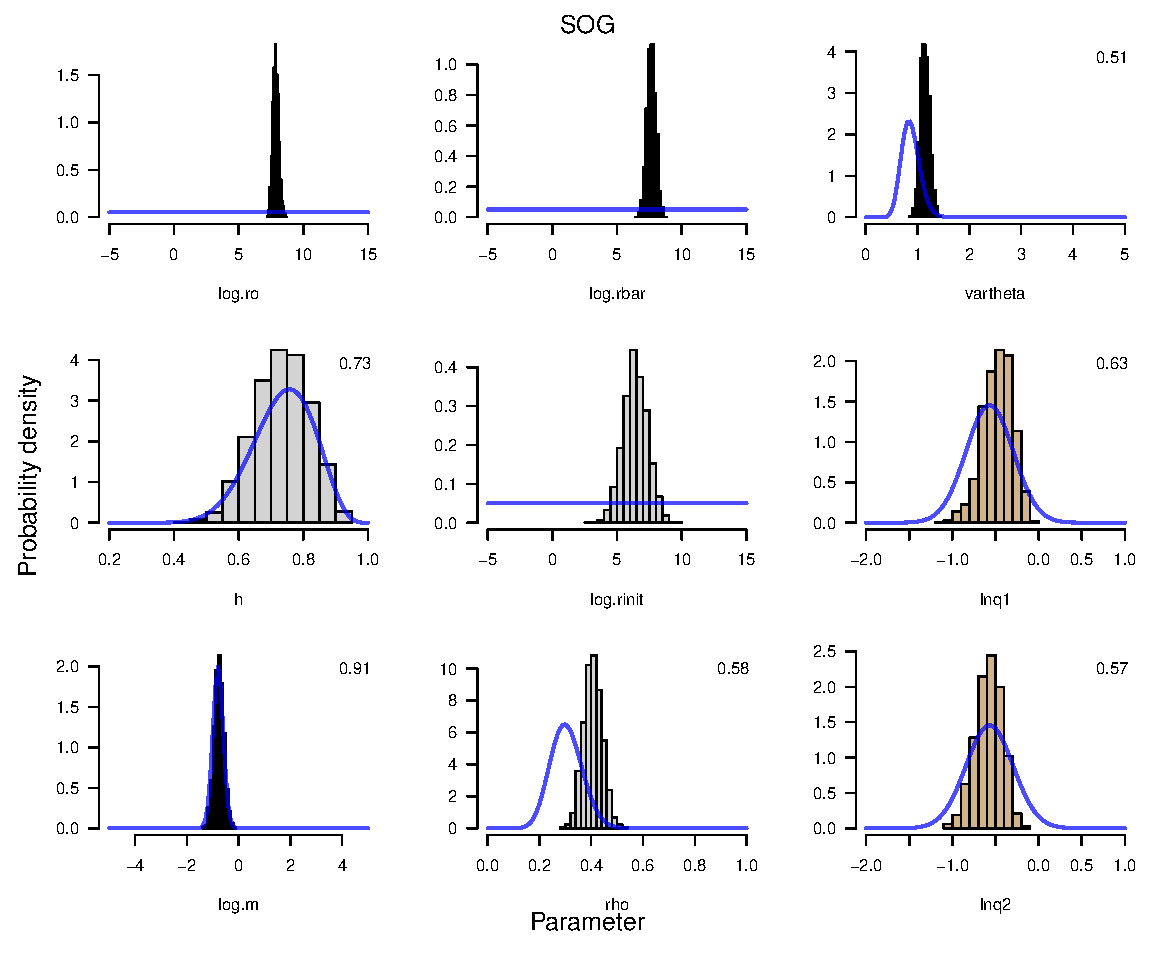
\includegraphics[scale=0.4]{../FIGS/qPriorFigs/iscam_fig_marginals_SOG}
		\caption{Strait of Georgia: Marginal \& prior distributions.}
	\end{figure}
\end{frame}
%% subsection diagnostics (end)

\subsection{Advice for management} % (fold)
\label{sub:advice_for_management}
%
\begin{frame}[t,shrink=35]\frametitle{Forecast: Old cutoffs}
	% latex.default(xTable, file = fn, rowname = NULL, longtable = FALSE,      landscape = FALSE, cgroup = cgrp, n.cgroup = ncgrp, caption = cap,      label = "TableCatchAdvice", na.blank = TRUE, vbar = FALSE,      size = "small") 
%
\begin{table}[!tbp]
 \small
 \caption{Estimated spawning stock biomass,  age-4+ biomass and pre-fishery
			biomass for poor average and good recruitment, old cutoffs,  and 
			available harvest based on median values from the joint posterior distribution.\label{TableCatchAdviceOldCuttoffs}} 
 \begin{center}
 \begin{tabular}{lllclllclclll}\hline\hline
\multicolumn{3}{c}{\bfseries }&
\multicolumn{1}{c}{\bfseries }&
\multicolumn{3}{c}{\bfseries Pre-fishery forecast biomass}&
\multicolumn{1}{c}{\bfseries }&
\multicolumn{1}{c}{\bfseries }&
\multicolumn{1}{c}{\bfseries }&
\multicolumn{3}{c}{\bfseries Available harvest}
\tabularnewline \cline{1-13}
\multicolumn{1}{c}{Stock}&\multicolumn{1}{c}{SSB}&\multicolumn{1}{c}{4+ Biomass}&\multicolumn{1}{c}{}&\multicolumn{1}{c}{Poor}&\multicolumn{1}{c}{Average}&\multicolumn{1}{c}{Good}&\multicolumn{1}{c}{}&\multicolumn{1}{c}{Cutoff}&\multicolumn{1}{c}{}&\multicolumn{1}{c}{Poor}&\multicolumn{1}{c}{Average}&\multicolumn{1}{c}{Good}\tabularnewline
\hline
HG&16,579& 7,089&& 9,618&12,892&21,478&&10,700&&     0& 2,192& 4,296\tabularnewline
PRD&27,046&20,593&&24,150&27,492&37,286&&12,100&& 4,830& 5,498& 7,457\tabularnewline
CC&14,666& 7,809&&11,357&14,709&22,883&&17,600&&     0&     0& 4,577\tabularnewline
SOG&125,261& 72,937&& 94,703&112,856&138,448&& 21,200&& 18,941& 22,571& 27,690\tabularnewline
WCVI&14,679& 8,267&&15,321&20,906&31,130&&18,800&&     0& 2,106& 6,226\tabularnewline
\hline
\end{tabular}

\end{center}

\end{table}


\end{frame}
%
\begin{frame}[t,shrink=35]\frametitle{Forecast: New cutoffs}
	% latex.default(xTable, file = fn, rowname = NULL, longtable = FALSE,      landscape = FALSE, cgroup = cgrp, n.cgroup = ncgrp, caption = cap,      label = "TableCatchAdvice", na.blank = TRUE, vbar = FALSE,      size = "small") 
%
\begin{table}[!tbp]
 \small
 \caption{Estimated spawning stock biomass,  age-4+ biomass and pre-fishery biomass for poor average and good recruitment, new cutoffs (based on median value of 0.25\bo\ estimated within the \iscam\ model), and available harvest based on the median values from the joint posterior distribtuion.\label{TableCatchAdviceNewCuttoffs}} 
 \begin{center}
 \begin{tabular}{lllclllclclll}\hline\hline
\multicolumn{3}{c}{\bfseries }&
\multicolumn{1}{c}{\bfseries }&
\multicolumn{3}{c}{\bfseries Pre-fishery forecast biomass}&
\multicolumn{1}{c}{\bfseries }&
\multicolumn{1}{c}{\bfseries }&
\multicolumn{1}{c}{\bfseries }&
\multicolumn{3}{c}{\bfseries Available harvest}
\tabularnewline \cline{1-13}
\multicolumn{1}{c}{Stock}&\multicolumn{1}{c}{SSB}&\multicolumn{1}{c}{4+ Biomass}&\multicolumn{1}{c}{}&\multicolumn{1}{c}{Poor}&\multicolumn{1}{c}{Average}&\multicolumn{1}{c}{Good}&\multicolumn{1}{c}{}&\multicolumn{1}{c}{Cutoff}&\multicolumn{1}{c}{}&\multicolumn{1}{c}{Poor}&\multicolumn{1}{c}{Average}&\multicolumn{1}{c}{Good}\tabularnewline
\hline
HG&16,579& 7,089&& 9,618&12,892&21,478&&10,436&&     0& 2,456& 4,296\tabularnewline
PRD&27,046&20,593&&24,150&27,492&37,286&&19,641&& 4,510& 5,498& 7,457\tabularnewline
CC&14,666& 7,809&&11,357&14,709&22,883&&15,600&&     0&     0& 4,577\tabularnewline
SOG&125,261& 72,937&& 94,703&112,856&138,448&& 35,013&& 18,941& 22,571& 27,690\tabularnewline
WCVI&14,679& 8,267&&15,321&20,906&31,130&&14,894&&   427& 4,181& 6,226\tabularnewline
\hline
\end{tabular}

\end{center}

\end{table}


\end{frame}
% subsection advice_for_management (end)

\subsection{Outstanding issues} % (fold)
\label{sub:outstanding_issues}
\begin{frame}[t]\frametitle{Outstanding issues}
	\begin{itemize}
		\item<+-> Reference points (e.g., B$_0$) based on non-stationary parameters (e.g., $M_t$, selectivity, growth).
		\item<+-> Strong retrospective bias in PRD.
		\item<+-> Formal evaluation of alternative hypotheses.
	\end{itemize}
\end{frame}

% subsection outstanding_issues (end)
% section part_ii (end)
